\documentclass[12pt, oneside, a4paper]{article}

\usepackage[all]{xy}
\usepackage[english]{babel}
\usepackage[T1]{fontenc}
\usepackage{amsthm, amsmath, amssymb, amsfonts, color, hyperref}
\usepackage{graphicx}
\usepackage{amsthm}
\usepackage{amsbsy}
\usepackage{amssymb}
\usepackage{amsfonts}
\usepackage{abstract}
\usepackage{multirow,rotating,array}
\usepackage[dvips]{lscape}

\def\cX{\ensuremath{\mathcal{X}}}
\def\cY{\ensuremath{\mathcal{Y}}}
\def\cF{\ensuremath{\mathcal{F}}}
\def\bP{\ensuremath{\mathbb{P}}}
\newcommand{\BigChar}[1]{\parbox{11pt}{\HUGE #1}}
\theoremstyle{plain}
\newtheorem{theorem}{Theorem}[section]
\newtheorem{proposition}[theorem]{Proposition}
\newtheorem{lemma}[theorem]{Lemma}
\newtheorem{corollary}[theorem]{Corollary}
\newtheorem{remark}[theorem]{Remark}
\newtheorem{definition}[theorem]{Definition}
\newtheorem{notation}[theorem]{Notation}
\def\indep{\perp\!\!\!\perp}
\newcommand{\given}{\mbox{ }\vert\mbox{ }}
\newcommand{\F}{\mathcal{F}}
\newcommand{\E}{\mathbb{E}}
\renewcommand{\P}{\mathbb{P}}
\newcommand{\R}{\mathbb{R}}
\newcommand{\X}{\mathcal{X}}
\newcommand{\B}{\mathcal{B}}
\newcommand{\V}{\mathbb{V}}
\newcommand{\Y}{\mathcal{Y}}
\newcommand{\TV}[1]{\left|\left| #1 \right|\right|_{TV}}
\newcommand{\email}[1]{\href{mailto:#1}{#1}}
\newcommand{\loss}{\ell(Y,f(X))}
\renewcommand{\hat}[1]{\widehat{#1}}
\newcommand{\RademacherVariable}{\sigma}
\newcommand{\RademacherComplexity}{\mathfrak{R}}
\newcommand{\bs}[1]{\boldsymbol{#1}}
\DeclareMathOperator*{\argmin}{argmin}
\DeclareMathOperator*{\vcd}{\textsc{vcd}}
\DeclareMathOperator*{\sgn}{sgn}
\newcommand{\indicator}{\mathbf{1}}
\renewcommand{\ref}[1]{(\ref{eq:#1})}
\newcommand{\mnorm}[1]{\ell\left(#1\right)}
%\newcommand{\mnorm}[1]{\left|\left| #1\right|\right|}
\newcommand{\riskmom}{\sqrt[q]{R_n^q(f)}}
\newcommand{\stock}{IBM}
\renewcommand{\qedsymbol}{$\blacksquare$}

\newcommand{\Pn}{\P^n}
\newcommand{\Pd}{\P_1}
\newcommand{\Yij}[2]{Y_{#1:#2}}
\newcommand{\Yin}{\Yij{1}{n}}
\newcommand{\Sij}[2]{\sigma_{#1:#2}}
\newcommand{\Sin}{\Sij{1}{n}}
\newcommand{\Sprod}[4]{\Sij{#1}{#2}\otimes\Sij{#3}{#4}}
\newcommand{\Pij}[2]{\P_{#1:#2}}
\newcommand{\Pin}{\Pij{1}{n}}
\newcommand{\Pot}[4]{\P_{#1:#2\otimes #3:#4}}
\newcommand{\Pprod}[4]{\Pij{#1}{#2}\otimes\Pij{#3}{#4}}
\newcommand{\Yinf}{Y_\infty}
\newcommand{\Sinf}{\sigma_\infty}
\newcommand{\Pinf}{\P_\infty}
\newcommand{\Pini}{\P_{1:n+1}}
\newcommand{\Yini}{\Yij{1}{n+1}}


\newcommand{\bb}[1]{\textbf{#1}}

\newtheorem{thm}{Theorem}[section]
\newtheorem{lem}[thm]{Lemma}
\newtheorem{prop}[thm]{Proposition}
\newtheorem{cor}[thm]{Corollary}
%\newtheorem{clm}[thm]{Claim}

\theoremstyle{definition}
\newtheorem{dfn}[thm]{Definition}
\newtheorem{rem}[thm]{Remark}
%\newtheorem*{remu}{Remark}
\newtheorem{ex}[thm]{Example}
\newtheorem{exs}[thm]{Examples}
\newtheorem{assumption}{Assumption}
\newtheorem{metaphor}{Metaphor}
\newtheorem{idea}{Idea}
\newtheorem{convention}{Convention}

\def \grad {\overrightarrow{\nabla}}
\def \curl {\overrightarrow{\nabla} \wedge \cdot}
\def \div {\overrightarrow{\nabla} \cdot}
\def \nab {\ensuremath{\nabla}}
\def \im {\text{im }}
\def \ker {\text{ker }}
\def \det {\text{det }}
\def \trace {\text{tr }}


\def\deq{:=}
\def\reals{\mathbb{R}}
\def\naturals{\mathbb{N}}
\def \C {\mathcal{C}} % for categories
\def \D {\mathcal{D}}
\def \S {\mathcal{S}}
%\def \P {\mathcal{P}}
\def \cX{\mathcal{X}}
\def \var{\mathrm{var}}
\def\pr{\ensuremath{\mathbb{P}}}
\def\Ebb{\ensuremath{\mathbb{E}}}
\def\expectation{\ensuremath{\mathbb{E}}}
\def\abcd{\ensuremath{\begin{pmatrix}a & b \\ c & d \end{pmatrix}}}
\def\Cbb{\ensuremath{\mathbb{C}}}
\def\Kbb{\ensuremath{\mathbb{K}}}
\def\Nbb{\mathbb{N}}
\def\Pbb{\mathbb{P}}
\def\Qbb{\mathbb{Q}}
\def\Rbb{\ensuremath{\mathbb{R}}}
\def\Hbb{\ensuremath{\mathbb{H}}}
\def\Halfplane{\ensuremath{\mathbb{H}^{2} = \left\lbrace z = x + iy \in \mathbb{C}
 \;|\; y = \mathrm{Im} z \gt 0 \right\rbrace}}
\def\MaxCompact{\ensuremath{\begin{pmatrix}\cos\varphi & -\sin\varphi \\ \sin\varphi & \cos\varphi\end{pmatrix}}}
\def\gg{\ensuremath{\mathfrak{g}}}
\def\SL{\ensuremath{SL(2,\Rbb)}}
\def\sl{\ensuremath{\mathfrak{sl}(2,\Rbb)}}
\def \eps {\varepsilon}
\def \AA{\ensuremath{\mathcal{A}^{1}}}
\def  \AAA{\ensuremath{\mathcal{A}}}
\def \Fff{\mathfrak{F}}
%\def \commutes {\ar@{}[rd]|{\circlearrowleft}}
\def \commutes {\ar@{}[rd]|{\mbox{ \Large{$\circlearrowleft$} }}}

\newcommand{\tensor}{\otimes}
\newcommand{\gt}{>}
\newcommand{\lt}{<}
\newcommand{\itexarray}[1]{\begin{matrix}#1\end{matrix}} %To draw commutative Diagrams
\newcommand{\Ob}{{\rm Ob}}
     \newcommand{\Cob}{{\rm Cob}}   
	\newcommand{\Vect}{{\mathrm{Vect}}}   
	\newcommand{\Hilb}{{\mathrm{Hilb}}}    
	\newcommand{\tr}{{\rm tr}}   
      \newcommand{\Hom}{{\rm hom}}
\newcommand{\cChVect}{\mathrm {cCh(Vect)}}
\newcommand{\gVect}{\mathrm {gVect}} 
\newcommand{\To}{\Rightarrow}  
\newcommand{\newword}[1]{\textbf{\emph{#1}}}

\title{An introduction to the Concentration of Measure and Empirical Process Theory}
\author{Peadar Coyle}

\begin{document}

\renewcommand{\baselinestretch}{1.5}

\maketitle
\tableofcontents
\listoffigures
\newpage
\section{Acknowledgements}
Writing a thesis is a difficult endeavour, and one often wonders if the work is worth it. 
However seeing the fruits of your labour and remembering that you have learned some wonderful Mathematics - makes it all 
worth it. I ended up doing this thesis - in Mathematics due to what seems like a stochastic process - ending up in Luxembourg
was not in my plan. However I am grateful to the staff at the University, for all their guidance and support over the past few years.
I am also grateful to the Machine Learning experts I spoke to during my Internship at Amazon.com and Import.io, I would never
have written this thesis if I hadn't been exposed to the reality of \textit{beautiful industrial applications} of statistics and
probability theory. I am deeply grateful to Professor Pecatti for his sense of humour (essential when working with me) 
and inspiring me to learn about Sudakov-Fernique Inequalities\footnote{The acorn of this thesis was in a Mathematics
Seminar given by the author last year on a particular Concentration Inequality called the Sudakov-Fernique Inequality\cite{Chatterjee2005}}.
\paragraph{} Early drafts of this thesis were read by a Mr Daniel Rowlands and a Dr Robert Horton - I am very grateful
that my statistically literate friends could help me solidify my ideas and presentation, writing often feels like a lonely
process and community support is invaluable. I also thank my various mentors and friends - Ben, Gregorio, Usman, Matt,
Alan, Pierre, Miles, Mike, Alexander, Chris, Danielle, Arthur and all the others who I've forgotten to mention - I am very grateful for 
your discussions about Mathematics, Physics, Philosophy and life over the past few years.
Finally - I thank my girlfriend and family for all their help and support - it is always good to have someone remind you that there are
more important things than work. 
\newpage

\begin{center}
 \textit{For Audrey}
\\
\textit{Amare et sapere vix deo conceditur}
\end{center}

\flushleft
\newpage
\section{Notation}
We introduce some notation that is used throughout the paper. We assume
that $X_1, \cdots , X_n$ are independent random variables taking values in a
measurable space $\mathcal{X}$. Denote by $X_1^n$ the vector of these n random
variables. Let $f: \mathcal{X}^n \rightarrow \mathbb{R} $be some measurable function.
\begin{itemize}
 \item almost surely is denoted by a.s.
\item X,Y,Z refer to random variables.
\item $\mathbb{P}$ Probability distribution
\item $\mathbb{R,C}$ field of real and complex numbers respectively
\end{itemize}
\newpage
\section{Introduction}
In this thesis we will introduce some aspects from Empirical process theory and Concentration of Measure. We are interested in applications in Learning 
theory but do not have the time nor the scope to introduce model theory and VC-theory. Our aims are more modest, we want to introduce some concentration
inequalities, show their applications in Empirical process theory and mention in passing some Statistical Learning theory. We will not be able to 
introduce all of these complex notions and we refer to the literature when we feel it is good to do so.  
Our first subsection will introduce Concentration of Measure and in passing we will see some of the celebrated theorems and inequalities. Elsewhere in 
thesis we will examine these theorems in more detail readers who are already familiar with the theorems - or perhaps Computer Scientists can just read
the introduction and move to the end. 
The style of this paper will be mostly aimed at pure mathematicians - so the standard of rigor is high. I have endeavoured to add my own opinions about
what is difficult and what is easy, and elucidate some of these \textit{unoriginal} and classical proofs. Most of what is reproduced here can be found 
in other textbooks or seminars, but the aim here is to condense as many of these as possible and rewrite them for an applied Statistician or Machine 
Learning expert audience. 
\paragraph{} Let us suppose that we have a large number of scalar random variables $X_1, \cdots,X_n$, which have a bounded 
size on average (e.g. their mean and variance would be O(1)). An interesting and important question is
what can one say about their sum? $S = X_1 + \cdots + X_n$? If each individual sumand $X_i$ varies in an interval
of size O(1), then their sum of course varies in an interval of size $0(n)$. However a remarkable phenomenon,
known as \textit{concentration of measure}, asserts that assuming a sufficient amount of independendence between the 
component variables $X_1, \cdots,X_n$, this sum sharply concentrates to a much narrower range, typically an interval
of size $O(\sqrt{n})$. This phenomenon is quantified by a variety
 of \textit{large deviation inequalities}\footnote{Roughly speaking
, large deviations theory concerns itself with the exponential decline of probability measures of certain kinds of extreme
or tail events as the number of observations grows large see \cite{Touchette20091, LargeDeviations} for further details. 
Readers interested in a thorough introduction can read from the \textit{"Mozart"} of large deviations theory \cite{varadhan2008}}
that give upper bounds (often exponential in nature) on the probability that such a combined random variable deviates significantly 
from its mean. The same phenomenon applies not only to linear expressions such as $S = X_1 + \cdots + X_n$, but more 
generally to nonlinear combinations $F(X_1, \cdots,X_n)$ of such variables, provided that the nonlinear function F is sufficiently 
regular - for example Lipschitz. 
\paragraph{} The basic intuition is that independent random variables find it difficult to "work together" to 
simultaneously pull a sum $S = X_1 + \cdots + X_n$ or a more general combination $F(X_1, \cdots,X_n)$ too far from its' mean.
Independendence is the key here; concentration of measure results typically fail if the $X_i$ are too highly concentrated
to each other. Although such results do exist see for example the work by Kontorovich on Mixing Phenomenoa \cite{Kontorovich_Metric}
or \cite{McDonald_TimeSeries} for work using time series data. 
\paragraph{} There are many applications of concentration of the concentration of measure phenomenon, such as random 
matrix theory, but we will mostly focus on applications in Computer Science not Physics\footnote{Ironic perhaps, since the author
once studied in a Physics department}. We wholeheartedly recommend the excellent book by Terry Tao on Random Matrix
Theory \cite{tao2012topics}. \footnote{For an excellent result relating to concentration inequalities in Random Matrix theory
I recommend \cite{Tropp_FoCM_2011}, it truly is amazing to see the power of Concentration of Measure}
\paragraph{} Assuming that one has a sufficient amount of independence, the concentration of measure tends to be
sub-gaussian in nature, this probability that one is at least $\lambda$ standard deviations (s.d.) from the mean tends
to drop off like $C\exp({-c\lambda^2})$ for some C,c $\gt 0$. In particular, one is $O(\log^{\dfrac{1}{2}}n)$ standard deviations
from the mean with overwhelming probability. Indeed, concentration of measure is our primary tool for ensuring that various
events hold with overwhelming probability.
\subsection{What does the word Application mean?}
The word \textit{applications} means different things to different people. If we wear our Mathematican hats we are always looking 
for a new tool to prove some theorem. Or reprove a celebrated theorem in a new way. 
Computer Scientists are always concerned with algorithms and performanace analysis and statisticians or
 \textit{data scientists}\footnote{It will be an interesting test case for the durability of job titles in industrial applications
of Mathematics to see if the term data scientist is dated in 5 years.} are after getting a handle on the 
asymptotics of estimators and samplers. 
In short, each specialist wants to know what a given tool will contribute to his field. 
\paragraph{} The remarkable thing about concentration of measure is that is uses span a wide range - from something practical as decoding neural signals to esoteric topics such as analyzing convex bodies in Banach spaces. 
It is too much to go beyond one or two applications.
So I'll cite some here 
\begin{itemize}
\item  Milman's proof of Dvoretzky's theorem on sections of convex bodies\cite{Milman}
\item a widely cited lemma of Johnson and Lindenstrauss concerning low-distortion dimensionality reduction in $\mathbb{R}^{n}$ by random projections\cite{JordanLipschitz}.
\item Applications in Economic Forecasting\cite{McDonald_TimeSeries}.
\item Statistics and empirical processes and machine learning\cite{SLT_Lugosi_Bocheron}
\end{itemize}
In the interest of keeping this document short we shall only look at the last example.
\subsection{What is in this thesis?}
In section \ref{sec:ConcMeasure} we give a rapid overview of concentration of measure including
some of the more advanced methods like the Herbst argument which will not be used in the thesis. 
In section \ref{sec:SLT} we will introduce someof the language from applications in statistical learning theory
including in particular empirical process theory. In the following section we include some remarks about Machine Learning
and Artificial Intelligence, this is just to motivate the thesis\ref{sec:MachineLearning}.
\paragraph{} In \ref{sec:ConcInequalities} we introduce the major concentration inequalities
(we refer the reader for further details to \cite{Ledoux_lecture_notes}) which 
we shall use - we start with Hoeffding and then introduce a few variants and finally the celebrated McDiarmid Inequality\cite{McDiarmid_1997}
- which we will use to prove results in the applications section. In \ref{sec:Applications} we return to our applications -
and give a more rigorous and complete introduction to our chosen subfield of Statistical Learning Theory - this will be of
particular interest to Mathematicans who may not be familiar with the language. The remainder of the \ref{sec:Applications} introduces
the celebrated Vapnik-Chervonenkis dimnesion.
In \ref{sec:Rademacher} we introduce the meat of the applications through the technique of Rademacher averages, we 
end the section by elucidating on the difficulty of calculating such averages - in learning theory through the lens of
empirical risk. We follow this up by considering dependent data in \ref{sec:dependence}.
After reminding the reader of the language of time series \cite{mcquarrie1998regression, romer2011advanced} we explicitly 
calculate some Risk bounds using the language of VC theory and Rademacher \ref{sec:risk-bounds} and then consider
this for a fixed-memory model from Econometrics \ref{sec:fixed-memory}. 
Finally in \ref{sec:Discussion} we end the thesis with some discussion and bibliographic remarks. 

\section{What are other examples of Concentration of Measure?}\label{sec:ConcMeasure}
We have already met the intuitive idea of \textit{concentration of measure} let us make this more mathematical.
 Let $X$ be a random variable taking values in some metric space $\mathsf{X}$. Then we say that 
the distribution of $X$ has the concentration property if, 
for any set $A \subset \mathsf{X}$ such that $\mathbb{P}(X \in A) \ge 1/2$, we have

\begin{equation}\label{eq:1} {\mathbb P}\left( d(X,A) \le r\right) \xrightarrow{r \rightarrow \infty} 1. \end{equation}
where r is a constant and $\mathbb{P}$ is some unknown probability distribution. 
Here, $d(x,A)$ is the distance from the point $x \in \mathsf{X}$ to the set $A$:

\begin{equation*} d(x,A) := \inf_{y \in A} d(x,y). \end{equation*}

Another way to express $\ref{eq:1}$ is as follows: for any set $A \subset \mathsf{X}$ and any $r \ge 0$, define the $r$-blowup of $A$ by

\begin{equation*} A_r := \left\{ y \in {\mathsf X}: d(y,A) \le r \right\} \equiv \left\{ y \in {\mathsf X}: \exists x \in A \text{ such that } d(x,y) 
\le r \right\}. \end{equation*}

Then $X$ has the concentration property if

\begin{equation*} {\mathbb P}(X \in A) \ge 1/2 \quad \Longrightarrow \quad 
\lim_{r \rightarrow \infty} {\mathbb P}(X \in A_r) = 1.\end{equation*}

In other words, $X$ has the concentration property if any set containing $X$
 with not too small a probability can be “blown up” to contain $X$ with near-certainty.

Here are two classic examples of concentration:
\begin{itemize}
    \item \textbf{Gaussian distribution in Euclidean space.}
 Let $\mathsf{X} = \mathbb{R}^n$ and take $d(x,y) = \| x - y \|_2$ — the usual Euclidean distance. Let {X} be a standard $n$-dimensional Gaussian random variable, i.e., $X \sim N(0,I_n)$, where $I_n$ is the $n\times n$ identity matrix. Then for any $r \ge 0$ we have

    \begin{equation*} {\mathbb P}(X \in A) \ge 1/2 \quad \Longrightarrow \quad {\mathbb P}(X \in A_r) \ge 1 - e^{-r^2/2}. \end{equation*}
    \item \textbf{Uniform distribution in Hamming space.}
 Let $\mathsf{X}$ be the Hamming cube ${\{0,1\}^n}$ equipped with the normalized Hamming distance

    \begin{equation*} d(x,y) = \frac{1}{n}\sum^n_{i=1}1_{\{x_i \neq y_i\}} \end{equation*}

    that counts the fraction of bits in which $x = (x_1,\ldots,x_n)$ and 
$y = (y_1,\ldots,y_n)$ disagree. Let $X$ have the uniform distribution on $\{0,1\}^n$, i.e., 
$\mathbb{P}(X=x) = 2^{-n}$ for all $x$. Then

\begin{equation*} \mathbb{P}(X \in A) \ge 1/2 \quad \Longrightarrow \quad \mathbb{P}(X \in A_r) \ge 
1 - e^{-2nr^2}.\end{equation*}l
\end{itemize}
These two examples suggest that we should aim for 
“hard” statements in the form of sharp bounds on the concentration function

\begin{equation*}\alpha_X(r) := \sup_{A:\, {\mathbb P}(X \in A) \ge 1/2} {\mathbb P}(X \not\in A_r) \end{equation*}
as opposed to merely “soft” statements of the form $\alpha_X(r) \rightarrow 0$ as $r \rightarrow \infty$. The 64,000 pounds question is: how do we get such bounds?

There are two ways to accomplish this goal, and the main idea underlying these two ways is to replace sets with some other objects that are hopefully 
easier to handle. The first way is to replace sets by probability measures, the second is to replace them by functions. 

Fix a set $A \subset \mathsf{X}$ with $\Pr(X \in A) > 0$. Let $\mathbb{P}$ denote the distribution of $X$, and let 
$P_A$ denote the conditional distribution of $X$ given $X \in A$. That is, for any (measurable) set $B \subset \mathsf{X}$ we have

\begin{equation*} P_A(B) := \frac{P(A \cap B)}{P(A)}. \end{equation*}

I am using the subscript notation $\mathbb{P}_A$ instead of the more usual 
$\mathbb{P}(\cdot|A)$ to indicate the fact that $\mathbb{P}_A$ 
is a probability measure in its own right. In this way, we can associate to each non-null set $A$
a probability measure $\mathbb{P}_A$. 
Now, here is a very simple observation that turns out to be very consequential\footnote{In fact we call the following 
equation \textit{relative entropy} or \textit{Kullback-Leibler} distance -
 we recommend that readers interested in Information Theory look at \cite{cover2006elements}. Unfortunately
it is beyond the scope of this thesis to introduce all the nomeclature from Information Theory.}:

\begin{equation}\label{eq:2}
 D(\mathbb{P}_A \| \mathbb{P}) = \log \frac{1}{\mathbb{P}(A)}.\end{equation}

This is very easy to prove: for any set $B$ we have

\begin{equation} \mathbb{P}_A(B) = \frac{1}{\mathbb{P}(A)}\int_B 1_A(x) \mathbb{P}(dx), \end{equation}
so $\mathbb{P}_A$ is absolutely continuous with respect to $\mathbb{P}$ with the Radon-Nikodym derivative 
\begin{equation*}d\mathbb{P}_A/d\mathbb{P} = 1_A/\mathbb{P}(A)\end{equation*}. Therefore, by definition of the divergence,

\begin{equation*} 
D(\mathbb{P}_A \| \mathbb{P}) = \int d\mathbb{P}_A \log \frac{d\mathbb{P}_A}{d\mathbb{P}} = \frac{1}{\mathbb{P}(A)}\int_A d\mathbb{P} \log\frac{1}{\mathbb{P}(A)} = \log \frac{1}{\mathbb{P}(A)}. \end{equation*}

So if we are interested in bounding the probabilities of various sets $A$, we may hope to get some mileage out of 
the relationship $\ref{eq:2}$.

On the other hand, we may also associate to a set $A$ with $\mathbb{P}(A) > 0$ the function

\begin{equation*} f_A(x) := d(x,A) \equiv \inf_{y \in A} d(x,y). \end{equation*}

This function is Lipschitz: for any $x,x' \in \mathsf{X}$,

\begin{equation*}f_A(x) - f_A(x') = \inf_{y \in A}d(x,y) - \inf_{y \in A} d(x',y) \le \sup_{y \in A} \left[d(x,y) - d(x',y)\right] \le d(x,x'), 
\end{equation*}

where the last step is by the triangle inequality. Interchanging the roles of $x$ and $x'$, we get the Lipschitz property. Moreover, let us consider 
the random variable $Z = f_A(X)$, where $X$ is our original $\mathsf{X}$-valued random variable. Then we immediately notice two things:

    For any $r \ge 0$, $\mathbb{P}(Z \le r) = \mathbb{P}\left(d(X,A) \le r\right) = \mathbb{P}(A_r)$.
    If $P(A) = \mathbb{P}(X \in A) \ge 1/2$, then $0$ is a median of $Z$, in the sense that

    \begin{equation*} {\mathbb P}(Z \le 0) = \mathbb{P}(A) \ge 1/2 \qquad \text{and} \qquad {\mathbb P}(Z > 0) \ge 1/2 \end{equation*}

    (the second inequality is obviously true since $Z$ is nonnegative with probability $1$). 

These two observations suggest that we may obtain concentration bounds by bounding the probability that a given Lipschitz function of $X$ 
deviates from its median by more than $r$. In fact, it is easy to derive an alternative expression for the concentration function $\alpha_X$:

\begin{equation}\label{eq:3} \alpha_X(r) = \sup_{{\rm 1-Lipschitz\,} f} {\mathbb P}\Big( f(X) > m_f + r\Big), \end{equation}

where $m_f$ denotes any median of $f(X)$. We already showed, by passing from $A$ to $f_A = d(\cdot,A)$, that $\alpha_X$ is 
bounded from above by the quantity on the right-hand side of (\ref{eq:3}):

\begin{equation*} \alpha_X(r) = \sup_{A :\, P(A) \ge 1/2} {\mathbb P} \Big( f_A(X) > \underbrace{m_{f_A}}_{=0} + r \Big ) 
\le \sup_{{\rm 1-Lipschitz\,}f} {\mathbb P}\Big( f(X) > m_f + r\Big) \end{equation*}

To prove the reverse inequality, fix any $1$-Lipschitz function $f$ and consider the set $A_f : = \left\{ x \in \mathsf{X} : f(x) \le m_f \right\}$, 
where $m_f$ is any median of $f$. Then, by definition,

\begin{equation*} \mathbb{P}(X \in A_f) = \mathbb{P}\Big( f(X) \le m_f \Big) \ge 1/2. \end{equation*}

Moreover, if we consider the $r$-blowup

\begin{equation*} [A_f]_r = \Big\{ x \in {\mathsf X}: d(x,A_f) \le r \Big\}, \end{equation*}

then for any $x \in \mathsf{X}$ and any $y \in [A_f]_r$ we must have

\begin{equation*} f(x) - m_f \le f(x) - f(y) \le d(x,y), \end{equation*}

where the last step is by the Lipschitz property of $f$. Consequently, by definition of the concentration function,

\begin{equation*}  {\mathbb P}\Big( f(X) > m_f + r \Big) \le {\mathbb P}\Big( d(X,A_f) > r \Big) = 1 - P\left([A_f]_r\right) \le \alpha_X(r). 
\end{equation*}

By passing to the functional viewpoint, we obtain another equivalent characterization of the concentration property: a random variable {X} taking values in a metric space $(\mathsf{X},d)$ has the concentration property if real-valued Lipschitz functions $X$ are “nearly constant.”
\subsection{Probabilistic viewpoint}
Let’s look at the first, probabilistic viewpoint, which was born out of a 1996 breakthrough paper by Marton\cite{
marton1996measure}. Given a metric space $(\mathsf{X},d)$, 
let us define the $L_1$ Wasserstein distance (or transportation distance) between any two probability measures $P$ and $Q$ on it:

\begin{equation*} W_1(P,Q) := \inf_{X \sim P, Y \sim Q} {\mathbb E}[d(X,Y)], \end{equation*}

where the infimum is over all jointly distributed random variables $X,Y \in \mathsf{X}$, such that $P_X = P$ and $P_Y = Q$. Now consider a random 
variable $X \in \mathsf{X}$, for which we wish to establish concentration. What Marton showed is the following: Suppose the distribution $P$ of $X$ 
satisfies the $L_1$ transportation inequality

\begin{equation}\label{eq:4} W_1(P,Q) \le \sqrt{2c\, D(Q \| P)} \end{equation}

for some constant $c > 0$. Then $X$ has the concentration property, and moreover

\begin{equation*}  P(A) \ge 1/2 \quad \Longrightarrow \quad P(A_r) \ge 1 - \exp\left(- \frac{1}{2c}\left( r - \sqrt{2c \log 2}\right)^2 \right), 
\forall r > \sqrt{2 c \log 2}. \end{equation*} 

Marton’s proof is breathtakingly beautiful. Consider any two sets $A,B$ with $P(A),P(B) \neq 0$. 
Recalling our notation for conditional distributions, we can write

\begin{equation*} \begin{array}{rcl} W_1(P_A,P_B) &\le& W_1(P_A,P) + W_1(P_B,P) \\ &\le& \sqrt{2c\, D(P_A \| P)} + \sqrt{2c\, D(P_B \| P)} \\ &=& \sqrt{2c \log \frac{1}{P(A)}} + \sqrt{2c \log \frac{1}{P(B)}}, \end{array} \end{equation*}

where in the first step we have used the triangle inequality, in the second we have used the fact that $P$ 
satisfies the transportation inequality (\ref{eq:4}), and in the last step we have used the formula (\ref{eq:2}). 
Now suppose that $P(A) \ge 1/2$ and let $B = A^c_r$ for some $r$, where $c$ denotes set-theoretic complement. 
Then we can show that $W_1(P_A,P_B) \ge d(A,B) \ge r$. On the other hand,

\begin{equation*} \log \frac{1}{P(A)} \le \log 2 \qquad \text{and} \qquad \log\frac{1}{P(B)} = \log\frac{1}{1-P(A_r)}.
\end{equation*}
Combining these facts gives us the bound

\begin{equation*} r \le \sqrt{2c \log 2} + \sqrt{2c \log \frac{1}{1-P(A_r)}} \end{equation*}

that holds for all $r$. If $r > \sqrt{2 c \log 2}$, then we get

\begin{equation*} P(A_r) \ge 1 - \exp\left( - \frac{1}{2c}\left(r - \sqrt{2c \log 2}\right)^2\right),
\end{equation*}
so we indeed have concentration and a sharp bound on $\alpha_X(r)$, at least for large enough values of $r$.
 The main message here is that, in order to 
study concentration, it suffices to work on the level of probability measures and to focus one’s effort on showing that the distribution of $X$ 
satisfies a suitable transportation inequality. Since Marton’s original work, there have been many refinements and extensions, which I will not go into 
here. One such result, due to Sergey Bobkov and Friedrich Götze\cite{bobkov1999exponential}, says that $P$ satisfying a transportation inequality 
(\ref{eq:4}) is equivalent to 
the Gaussian concentration property

\begin{equation*} \alpha_X(r) \le e^{-r^2/2c}, \qquad \forall r \ge 0. \end{equation*}

Now let’s look at the complementary functional viewpoint. Recall that we seek tight upper bounds on deviation probabilities of the form

\begin{equation*} \mathbb {P}\Big( f(X) \ge m_f + r \Big), \qquad \forall r > 0. 
\end{equation*}
 It is easier to work with means instead of medians, and indeed it can be shown that concentration around the mean is equivalent to concentration
 around any median. So let’s focus on the mean. Let $X$, as before, be a random variable over some metric space $(\mathsf{X},d)$, and consider a
 Lipschitz function $f : \mathsf{X} \rightarrow \mathbb {R}$ such that $\mathbb{E}[f(X)] = 0$. 
 We can apply the well-known Chernoff trick: for any $r,\lambda > 0$ we have

\begin{equation*}\mathbb {P}\Big( f(X) \ge r \Big) = \mathbb{P}\Big( e^{\lambda f(X)} \ge e^{\lambda r} \Big) \le e^{-\lambda r} \mathbb{E}[e^{\lambda 
f(X)}]. \end{equation*}

Now the whole affair hinges on the availability of tight upper bounds on the logarithmic moment-generating function 
$\Lambda(\lambda) := \log \mathbb {E}[e^{\lambda f(X)}]$. 
The entropy method\cite{Raginsky_ConcMeasure,Ledoux_lecture_notes}, is the name for a set of techniques for bounding $\Lambda(\lambda)$ by means 
of various inequalities involving the relative entropy between various tilted distributions derived from
 $P$ and $P$ itself\footnote{We shall use $P$ and $\mathbb{P}$ interchangeable for the rest of this section. They both 
mean distribution}.

The entropy method has roots in the work of Michel Ledoux, who in turn distilled it from some very deep results of
 Michel Talagrand\cite{TalagrandInequality,Ledoux,Ledoux_lecture_notes}.

The simplest version of the entropy method goes something like this.
 Let us define, for any $t \in \mathbb{R}$, the tilted distribution $P^{(t)}$ via

\begin{equation*} \frac{dP^{(t)}}{dP}(x) = \frac{e^{tf(x)}}{e^{\Lambda(t)}} 
\end{equation*}

(assuming, of course, that $\Lambda(t)$ exists and is finite). Then we have

\begin{equation*} \begin{array}{rcl} D(P^{(t)} \| P) &=& \int dP^{(t)} \left[ tf - \Lambda(t)\right] \\ &=& \frac{1}{e^{\Lambda(t)}} t\, \mathbb{E}
\left[f(X)e^{tf(X)}\right] - \Lambda(t) \\ &=& t \Lambda'(t) - \Lambda (t) \\ &=& t^2 \frac{d}{dt} \left(\frac{\Lambda(t)}{t}\right). \end{array}
\end{equation*}


Integrating and using the fact that $\Lambda(0) = 0$, we get

\begin{equation}\label{eq:5} \Lambda(\lambda) = \lambda \int^\lambda_0 \frac{D(P^{(t)} \| P)}{t^2} dt. \end{equation}

Now suppose that we can bound $D(P^{(t)} \| P) \le ct^2/2$ for some $c > 0$. Then from (\ref{eq:5}) we have

\begin{equation*} \Lambda(\lambda) \le \frac{c\lambda^2}{2}, \qquad \forall t
\end{equation*}
which in turn gives the Gaussian tail bound

\begin{equation*} \mathbb{P}\Big( f(X) \ge r \Big) \le \inf_{\lambda > 0} \exp\left(-\lambda r + \frac{c\lambda^2}{2}\right) = \exp\left(-\frac{r^2}
{2c}\right). \end{equation*}

This is the so-called Herbst argument\cite{Ledoux_lecture_notes}. 
Of course, I have glossed over the most nontrivial part — 
namely, showing that we can bound the relative entropy $D(P^{(t)} \| P)$ by a quadratic 
function of $t$. I refer to \cite{Lugosi, Ledoux_lecture_notes,barvinok2005math} for 
further details.
\subsection{Some further classic examples}
Here is one classic example. 
Suppose that our function $f$ has the bounded difference property, i.e., there exist some constants $c_1,\ldots,c_n \ge 0$, such that changing the $i$-
th argument of $f$ while keeping others constant will change the value of $f$ by at most $c_i$:

\begin{equation*} \sup_{x_1,\ldots,x_n}\sup_{x'_i}\left| f(x_1,\ldots,x_i,\ldots,x_n) - f(x_1,\ldots,x'_i,\ldots,x_n) \right| \le c_i.
\end{equation*}
We can express this more succinctly as a Lipschitz property of $f$ if we define the weighted Hamming metric
\footnote{Readers interested in learning about Hamming metrics and Coding theory should refer to \cite{cover2006elements}}.

\begin{equation}\label{eq:6} d(x,y) = \sum^n_{i=1}c_i 1_{\{x_i \neq y_i\}} \end{equation}

(we can assume without loss of generality that all the $c_i$‘s are strictly positive, 
because we can simply ignore those coordinates of $x$ that do not affect the value of $f$). 
Then the bounded difference property is equivalent to saying that $f$ is $1$-Lipschitz with respect to 
this weighted Hamming metric. 
Moreover, it is possible to show that any product probability measure $P = P_1 \otimes \ldots \otimes P_n$ 
on the product space $\mathsf{X} = \mathcal{X}^n$ satisfies the transportation inequality

\begin{equation*} W_1(Q,P) \le \sqrt{2c\, D(Q \| P)}, \end{equation*}

where the Wasserstein distance is computed with respect to the weighted Hamming metric (\ref{eq:6}), 
and $c = \frac{1}{4}\sum^n_{i=1}c^2_i$. 
By the Bobkov–Götze result quoted above, this is equivalent to the concentration bound

\begin{equation*} \mathbb{P}\left( f(X) \ge \mathbb{E}[f(X)] + r \right) \le \exp\left( - \frac{r^2}{2c}\right) = 
\exp\left( - \frac{2r^2}{\sum^n_{i=1}c^2_i}\right).\end{equation*}

This is the well-known McDiarmid’s inequality\cite{McDiarmid_tutorial} - which we shall use a lot in this thesis.
What is important to state is that this inequality was originally derived using martingale techniques, but here we have arrived at it through a 
completely different route that took us back to where we started: concentration of Lipschitz functions around their means and/or medians, which (as we 
saw) is the same thing as the original, “stochastic-geometric” view of the concentration of measure phenomenon.
This \textit{equivalence} between \textit{concentration of Lipshitz functions} and \textit{"stochastic-geometric"} views of the concentration
of measure phenomenon is a very important general phenomenon, and important for proving new theorems or finding new insights in Probability Theory
or information theory\cite{cover2006elements}. For a thorough introduction to the uses of Concentration of Measure in Information theory we recommend
Raginsky \cite{Raginsky_ConcMeasure}. For other applications of concentration of measure we refer to \cite{boucheron2013concentration,
Ledoux_lecture_notes, Lugosi, SLT_Lugosi_Bocheron}. 
As mentioned before this work evolved out of some work on the Sudakov-Fernique inequality (in particular
a modern proof by Chaterjee\cite{Chatterjee2005}, readers who are familiar with
Stein inequalities and want to see some applications of Concentration Inequalities to Statistical Mechanics can refer to 
\cite{2009arXiv0906.1034C}
\subsection{What is Empirical Process theory}\label{sec:SLT}
The simplest example of an empirical process arises when trying to estimate a probability distribution from sample data. 
For those interested in applications it is worth highlighting that the \textit{data} could be from Economics - say we wanted to model when the next
recession would occur based on historical time-series data \cite{McDonald_TimeSeries} or it could be data from a 
social media website.
The difference between the empirical distribution function $F_n(x)$ and the true distribution function $F(x)$ converges to zero everywhere (by the law 
of large numbers), and — this is non- trivial — the maximum difference between the empirical and true distribution functions converges to zero, too (by 
the Glivenko-Cantelli theorem, a uniform law of large numbers). The "empirical process" $E_n(x)$ is the re-scaled difference, 
$n^{1/2}[F_{n}(x)−F(x)]$, and it converges to a Gaussian stochastic process that only depends on the true distribution (by the functional central limit 
theorem). 
\paragraph{} Empirical process theory is concerned with generalizing this sort of material to other stochastic processes determined by random samples, 
and indexed by infinite classes (like the real line, or the class of all Borel sets on the line, or some space parameterizing a regression model). The 
typical objects of concern are proving uniform limit theorems, 
and with establishing distributional limits. (For instance, one might one want to prove that the errors of all possible regression models in some class 
will come close to their expected errors, so that maximum-likelihood or least-squares estimation is consistent.) 
This endeavor is closely linked to Vapnik-Chervonenkis-style learning theory, and in fact one can see VC theory as an application of empirical process 
theory. So it is very difficult to untangle Vapnik-Chervonenkis(VC)-style learning theory from Concentration of Measure and Empirical Process theory.
Hence throughout this thesis you will see references to VC theory, and some of the celebrated theorems proven. It is worth highlighting that most of 
these areas are still active research areas - and you may encounter some 'simple' questions which are not easy to prove, or are in fact open questions.
But then we do live in the \textit{Golden age} of statistics and stochastic processes! 
Readers interested in more about Empirical Process theory should read 
\cite{vapnik2000nature,dudley1999uniform,massart,boucheron2013concentration} or the famous monograph \cite{Pollard1990}.
these all introduce the topic in more depth.
\subsection{So why should we care about empirical process theory?}\label{sec:MachineLearning}
Well let's say that you the reader are statistically literate, and you've 
learned some concentration of measure, and you have an interest in model selection - that is selecting among different mathematical 
model which all purport to describe the same data set. The basic strategy is to find conditions under which every model in a 
reasonable class will, with high probability, perform about as well on sample data as they can be expected to do on new data; this 
involves constraining the richness or flexibility of the model class.   

One of the \textit{buzzwords} in contemporary science is Machine Learning. We shall consider statistical learning a subtype of 
machine learning and leave the reader to form their own impressions of what machine learning is. 
Let us use the Vapnik notion of statistical learning for pedagogical reasons. We want to estimate some functional which depends on
an unknown distribution over a probability space X --it could be a \textit{concept}\footnote{In the machine learning sense},regression
coefficients, moments of the distribution, Shannon entropy, etc., even the distribution itself. We have a class of admissible distributions, called hypotheses, and a ``loss functional,'' an integral over X which tells us, for each hypothesis, how upset we should be when we guess wrong; this implicitly depends on the true distribution. Clearly we want the best hypothesis, the one which minimizes the loss functional --- but to explicitly calculate that we'd need to know the true distribution. 
Vapnik assumes that we have access to a sequence of independent random variables, all drawn from the 
(stationary) true distribution. What then are we to do?
\paragraph{}
One answer which I term the \textit{Vapnik answer} takes two parts.
 The first has to do with ``empirical risk minimization'': approximate the true, but unknown, loss 
functional, which is an integral over the whole space X, with a sum over the observed data-points, and go with the hypothesis that 
minimizes this ``empirical risk''; call this, though Vapnik doesn't, the ERM hypothesis. It's possible that the ERM hypothesis will do 
badly in the future, because we blundered into unrepresentative data, but we can show necessary and sufficient conditions for the loss 
of the ERM hypothesis to converge in probability to the loss of the best hypothesis. Moreover, we can prove that under certain very 
broad conditions, that if we just collect enough data-points, then the loss of the ERM hypothesis is, with high probability, within a 
certain additive distance (``confidence interval'' --- Vapnik's scare-quotes) of the loss of the best hypothesis. 
These conditions involve the Vapnik-Chervonenkis dimension, and a related quantity called the Vapnik-Chervonenkis entropy. 
Very remarkably, we can even calculate how much data we need to get a given approximation, at a given level of confidence, regardless 
of what the true distribution is, i.e. we can calculate distribution-independent bounds. (They do, however, depend on the nature of 
the integrands in the loss functional.)
\paragraph{}
These results about convergence, approximation, etc. are in essence extensions of the Law of Large Numbers to 
spaces of functions. As such the assumption that successive data-points are independent and 
identically distributed is key to the whole exercise. While it is possible to consider dependant data in Statistical learning
we shall not consider it in this thesis.
The second part of Vapnik's procedure is an elaboration of the first: For a given amount of data, we pick the hypothesis which 
minimizes the sum of the empirical risk and the ``confidence interval'' about it. This is termed by Vapnik - \textit{structural risk 
minimization} and shall not be considered in this thesis. I recommend \cite{vapnik2000nature} for further details. 



\section{Basic concentration inequalities via the martingale approach}
\label{section: Basic Concentration Inequalities}
\label{sec:ConcInequalities}
In the following section, some basic inequalities that are widely
used for proving concentration inequalities are presented, whose
derivation relies on the martingale approach. Their proofs convey
the main concepts of the martingale approach for proving concentration.
Their presentation also motivates some further refinements that are
considered in the continuation of this chapter.

\subsection{The Azuma-Hoeffding inequality}\label{subsection: Azuma's inequality}
The Azuma-Hoeffding inequality\footnote{The
Azuma-Hoeffding inequality is also known as Azuma's inequality.
Since it is referred numerous times in this chapter, it will be
named Azuma's inequality for the sake of
brevity.} is a useful concentration inequality for
bounded-difference martingales. It was proved in \cite{Hoeffding}
for independent bounded random variables, followed by a discussion
on sums of dependent random variables; this inequality was later
derived in \cite{Azuma} for the more general setting of
bounded-difference martingales. In the following, this inequality
is introduced.

\begin{thm}{\bf[Azuma-Hoeffding inequality]}
Let $\{X_k, \mathcal{F}_k\}_{k=0}^n$
be a discrete-parameter real-valued martingale sequence.
Suppose that, for every $k \in \{1, \ldots, n\}$, the condition
$ |X_k - X_{k-1}| \leq d_k$
holds almost surely (a.s.) for a real-valued sequence $\{d_k\}_{k=1}^n$ of
non-negative numbers. Then, for every $\alpha > 0$,
\begin{equation}
\pr( | X_n - X_0 | \geq \alpha) \leq 2 \exp\left(-\frac{\alpha^2}{2
\sum_{k=1}^n d_k^2}\right).
\label{eq: Azuma's concentration inequality - general case}
\end{equation}
\label{theorem: Azuma's concentration inequality}
\end{thm}

It is noted that Azuma's concentration inequality
is typically interpreted as $\frac{X_n - X_0}{\sqrt{n}}$ being sub-Gaussian.
The proof of the Azuma-Hoeffding inequality serves also
to present the basic principles on which the martingale
approach for proving concentration results is based.
Therefore, we present in the following the proof of this
inequality.

\begin{proof}
For an arbitrary $\alpha > 0$,
\begin{equation}
\pr(|X_n - X_0| \geq \alpha) = \pr(X_n - X_0 \geq \alpha) + \pr(X_n - X_0 \leq -\alpha).
\label{eq: union of disjoint events}
\end{equation}
Let $\xi_i \triangleq X_i - X_{i-1}$ for $i=1, \ldots, n$ designate
the jumps of the martingale sequence. Then, it follows by assumption that
$|\xi_k| \leq d_k$ and $\expectation[\xi_k \, | \, \mathcal{F}_{k-1}] = 0$
a.s. for every $k \in \{1, \ldots, n\}$.

From Chernoff's inequality,
\begin{eqnarray}
&& \pr(X_n - X_0 \geq \alpha) \nonumber \\
&& = \pr \Biggl(\sum_{i=1}^n \xi_i \geq \alpha \Biggr) \nonumber \\
&& \leq e^{-\alpha t} \, \expectation\left[\exp \left(t \sum_{i=1}^n \xi_i \right) \right],
\quad \forall \, t \geq 0.
\label{eq: Chernoff's inequality}
\end{eqnarray}
Furthermore,
\begin{align}\label{eq: smoothing theorem}
&& \expectation \biggl[ \exp \biggl(t \sum_{k=1}^n \xi_k \biggr)
\biggr] \nonumber \\
&& = \expectation \Biggl[ \expectation \biggl[ \exp \biggl(t
\sum_{k=1}^n \xi_k \biggr) \, | \, \mathcal{F}_{n-1} \biggr] \Biggr]
\nonumber \\
&& = \expectation \Biggl[ \exp \biggl(t \sum_{k=1}^{n-1} \xi_k
\biggr) \, \expectation \bigl[ \exp(t \xi_n) \, | \,
\mathcal{F}_{n-1} \bigr] \Biggr]
\end{align}
where the last equality holds since $Y \triangleq \exp \bigl(t
\sum_{k=1}^{n-1} \xi_k \bigr)$ is $\mathcal{F}_{n-1}$-measurable;
this holds due to fact that $\xi_k \triangleq X_k
- X_{k-1}$ is $\mathcal{F}_k$-measurable for every $k \in
\naturals$, and $\mathcal{F}_k \subseteq \mathcal{F}_{n-1}$ for $0
\leq k \leq n-1$ since $\{\mathcal{F}_k\}_{k=0}^{n}$ is a
filtration. Hence, the RV $\sum_{k=1}^{n-1} \xi_k$ and $Y$
are both $\mathcal{F}_{n-1}$-measurable, and
$\expectation[ XY | \mathcal{F}_{n-1}] =
Y \, \expectation[ X | \mathcal{F}_{n-1}].$

Due to the convexity of the exponential function, the straight line connecting
the end points of the function over the interval $[-d_k, d_k]$ lies
above this function. Since $|\xi_k| \leq d_k$ for every $k$
(note that $\expectation[\xi_k \, | \, \mathcal{F}_{k-1}] = 0$), it follows that
\begin{eqnarray}
&& \expectation \bigl[e^{t \xi_k} \, | \, \mathcal{F}_{k-1}\bigr] \nonumber \\
&& \leq \expectation \Bigl[\frac{(d_k + \xi_k) e^{t d_k} + (d_k-\xi_k) e^{-t d_k}}{2 d_k}
\, | \, \mathcal{F}_{k-1} \Bigr] \nonumber \\
&& = \frac{1}{2} \, \bigl(e^{t d_k} + e^{-t d_k} \bigr) \nonumber \\
&& = \cosh(t d_k).
\label{eq: cosine hyperbolic}
\end{eqnarray}
Since, for every integer $m \geq 0$,
$$(2m)! \geq (2m) (2m-2) \ldots 2 = 2^m \, m!$$
then, due to the power series expansions of the hyperbolic cosine and exponential functions,
$$\cosh(t d_k) = \sum_{m=0}^{\infty} \frac{(t d_k)^{2m}}{(2m)!}
\leq \sum_{m=0}^{\infty} \frac{(t d_k)^{2m}}{2^m \, m!} = e^{\frac{t^2 \, d_k^2}{2}}$$
which therefore implies that
$$ \expectation \bigl[e^{t \xi_k} \, | \, \mathcal{F}_{k-1}\bigr] \leq e^{\frac{t^2 \, d_k^2}{2}}.$$
Consequently, by repeatedly using the recursion in \ref{eq: smoothing theorem}, it follows
that
\begin{equation*}
\expectation \biggl[ \exp \biggl(t \sum_{k=1}^n \xi_k \biggr)
\biggr] \leq \prod_{k=1}^n \exp\left(\frac{t^2 \, d_k^2}{2}\right)
= \exp \left(\frac{t^2}{2} \, \sum_{k=1}^n d_k^2 \right)
\end{equation*}
which then gives (see \ref{eq: Chernoff's inequality}) that
\begin{equation*}
\pr(X_n - X_0 \geq \alpha) \leq
\exp\left(-\alpha t + \frac{t^2}{2} \, \sum_{k=1}^n d_k^2 \right), \quad \forall \, t \geq 0.
\end{equation*}
An optimization over the free parameter $t \geq 0$ gives that
$t = \alpha \left(\sum_{k=1}^n d_k^2\right)^{-1}$, and
\begin{equation}
\pr(X_n - X_0 \geq \alpha) \leq \exp \left(-\frac{\alpha^2}{2 \sum_{k=1}^n d_k^2} \right).
\label{eq: one-sided Azuma's inequality}
\end{equation}
Since, by assumption, $\{X_k, \mathcal{F}_k \}$ is a martingale with bounded jumps,
so is $\{-X_k, \mathcal{F}_{k}\}$ (with the same bounds on its jumps). This implies
that the same bound is also valid for the probability $\pr(X_n - X_0 \leq -\alpha)$
and together with \ref{eq: union of disjoint events} it completes the proof of
Theorem~\ref{theorem: Azuma's concentration inequality}.
\end{proof}

The proof of this inequality will be revisited later
in this chapter for the derivation of some refined versions,
whose use and advantage will be also exemplified.

\begin{rem}
In \cite[Theorem~3.13]{McDiarmid_tutorial}, Azuma's inequality is
stated as follows: Let $\{Y_k, \mathcal{F}_k\}_{k=0}^n$ be a
martingale-difference sequence with $Y_0=0$ (i.e., $Y_k$ is
$\mathcal{F}_k$-measurable, $\expectation[|Y_k|] < \infty$ and
$\expectation[Y_k| \mathcal{F}_{k-1}]=0$ a.s. for every $k \in
\{1, \ldots, n\}$). Assume that, for every $k$, there
exist some numbers $a_k, b_k \in \reals$ such that a.s.
$a_k \leq Y_k \leq b_k$. Then, for every $r \geq 0$,
\begin{equation}
\pr \left( \bigg|\sum_{k=1}^n Y_k\bigg| \geq r \right) \leq 2
\exp\left(-\frac{2r^2}{\sum_{k=1}^n (b_k-a_k)^2} \right).
\label{eq: concentration inequality for a martingale-difference
sequence (McDiarmid's tutorial)}
\end{equation}
As a consequence of this inequality, consider a discrete-parameter
real-valued martingale sequence $\{X_k, \mathcal{F}_k\}_{k=0}^n$
where $a_k \leq X_k - X_{k-1} \leq b_k$ a.s. for every $k$. Let $Y_k
\triangleq X_k - X_{k-1}$ for every $k \in \{1, \ldots, n\}$, so
since $\{Y_k, \mathcal{F}_k\}_{k=0}^n$ is a
martingale-difference sequence and $\sum_{k=1}^n Y_k = X_n - X_0$, then
\begin{equation}
\pr \left( |X_n - X_0| \geq r \right) \leq 2
\exp\left(-\frac{2r^2}{\sum_{k=1}^n (b_k-a_k)^2} \right), \quad \forall \, r > 0.
\label{eq: concentration inequality for a martingale sequence
(McDiarmid's tutorial)}
\end{equation}
\end{rem}

\begin{ex}
Let $\{Y_i\}_{i=0}^{\infty}$ be i.i.d. binary random variables
which get the values $\pm d$, for some constant $d>0$, with equal
probability. Let $X_k = \sum_{i=0}^k Y_i$ for $k \in \{0, 1,
\ldots, \}$, and define the natural filtration $\mathcal{F}_0
\subseteq \mathcal{F}_1 \subseteq \mathcal{F}_2 \ldots $ where
$$\mathcal{F}_k = \sigma(Y_0, \ldots, Y_k) \, , \quad \forall
\, k \in \{0, 1, \ldots, \}$$ is the $\sigma$-algebra that is
generated by the random variables $Y_0, \ldots, Y_k$. Note that
$\{X_k, \mathcal{F}_k\}_{k=0}^{\infty}$ is a martingale sequence, and
(a.s.) $ |X_k - X_{k-1}| = |Y_k| = d, \, \forall \, k \in
\naturals$. It therefore follows from Azuma's inequality that
\begin{equation}
\pr( | X_n - X_0 | \geq \alpha \sqrt{n}) \leq 2
\exp\left(-\frac{\alpha^2}{2d^2}\right). \label{eq: Azuma's
inequality for example1}
\end{equation}
for every $\alpha \geq 0$ and $n \in \naturals$. From the central
limit theorem (CLT), since the RVs
$\{Y_i\}_{i=0}^{\infty}$ are i.i.d. with zero mean and
variance~$d^2$, then
$\frac{1}{\sqrt{n}} (X_n - X_0) = \frac{1}{\sqrt{n}} \sum_{k=1}^n Y_k$
converges in distribution to
$\mathcal{N}(0,d^2)$. Therefore, for every $\alpha \geq 0$,
\begin{equation}
\lim_{n \rightarrow \infty} \pr( | X_n - X_0 | \geq \alpha
\sqrt{n})= 2 \, Q\Bigl(\frac{\alpha}{d}\Bigr)
\label{CLT1 - i.i.d. RVs}
\end{equation}
where
\begin{equation}
Q(x) \triangleq \frac{1}{\sqrt{2\pi}} \, \int_{x}^{\infty}
\exp\Bigl(-\frac{t^2}{2}\Bigr) \mathrm{d}t, \quad \forall \, x \in
\reals \label{eq: Q function}
\end{equation}
is the probability that a zero-mean and unit-variance Gaussian
Random Variable(RV) is larger than $x$. Since the following exponential
upper and lower bounds on the Q-function hold
\begin{equation}
\frac{1}{\sqrt{2\pi}} \, \frac{x}{1+x^2} \cdot e^{-\frac{x^2}{2}}
< Q(x) < \frac{1}{\sqrt{2\pi} \, x} \cdot e^{-\frac{x^2}{2}}, \;
\; \forall \, x>0 \label{eq: upper and lower bounds for the Q
function}
\end{equation}
then it follows from \ref{CLT1 - i.i.d. RVs} that the exponent
on the right-hand side of \ref{eq: Azuma's inequality for
example1} is the exact exponent in this example. \label{example1}
\end{ex}

\begin{ex}
In continuation to Example~\ref{example1}, let $\gamma \in (0,1]$,
and let us generalize this example by considering the case where the
i.i.d. binary RVs $\{Y_i\}_{i=0}^{\infty}$ have the
probability law
$$ \pr(Y_i = +d) = \frac{\gamma}{1+\gamma}, \quad \pr(Y_i =
-\gamma d) = \frac{1}{1+\gamma} \; .$$ Hence, it follows that the
i.i.d. RVs $\{Y_i\}$ have zero mean and variance $\sigma^2 =
\gamma d^2$. Let $\{X_k,
\mathcal{F}_k\}_{k=0}^{\infty}$ be defined similarly to
Example~\ref{example1}, so that it forms a martingale sequence.
Based on the CLT, $\frac{1}{\sqrt{n}} \, (X_n - X_0) =
\frac{1}{\sqrt{n}} \, \sum_{k=1}^n Y_k$ converges weakly to
$\mathcal{N}(0, \gamma d^2)$, so for every $\alpha \geq 0$
\begin{equation}
\lim_{n \rightarrow \infty} \pr( | X_n - X_0 | \geq \alpha
\sqrt{n})= 2 \, Q\biggl(\frac{\alpha}{\sqrt{\gamma} \, d}\biggr).
\label{eq:CLT2 - i.i.d. RVs}
\end{equation}
From the exponential upper and lower bounds of the Q-function in
\ref{eq: upper and lower bounds for the Q function}, the
right-hand side of \ref{eq:CLT2 - i.i.d. RVs} scales exponentially
like $e^{-\frac{\alpha^2}{2 \gamma d^2}}$. Hence, the exponent in
this example is improved by a factor $\frac{1}{\gamma}$ as
compared Azuma's inequality (that is the same as in
Example~\ref{example1} since $|X_k - X_{k-1}| \leq d$ for every $k
\in \naturals$). This indicates on the possible refinement of
Azuma's inequality by introducing an additional constraint on the
second moment. This route was studied extensively in the
probability literature, and it is studied along with Bernstein inequalities\cite{Bernstein} (that is 
inequalities which focus on the second moment) in \cite{Ledoux,boucheron2013concentration}. We shall
not consider such examples in this thesis. 
\label{example2}
\end{ex}

\subsection{McDiarmid's inequality}
\label{subsection: McDiarmid's inequality}
The following useful inequality is due to McDiarmid
(see Theorem 3.1 in(\cite{McDiarmid_1997} or
\cite{McDiarmid_tutorial}),
and its original derivation uses the martingale approach for its
derivation. We will relate, in the following, the derivation of this
inequality to the derivation of the Azuma-Hoeffding inequality
(see the preceding subsection). In some sense we can say that McDiarmid's
inequality generalizes the simple concentration inequality which we've seen before like \cite{Azuma}
to functions that depend on independently identically distributed (i.i.d.) random variables. 

\begin{thm}{\bf[McDiarmid's inequality]}
Let $\{X_k\}_{k=1}^n$ be independent real-valued random variables,
taking values in the set
$\mathcal{X} \deq \prod_{k=1}^n \mathcal{X}_k \subseteq \reals^n$.
Let $g: \mathcal{X} \rightarrow \reals$ be a measurable function
such that, for some constants $\{d_k\}_{k=1}^n$,
\begin{equation}
\bigl| g(\underline{x}) - g(\underline{x}') \bigr| \leq d_k,
\quad \forall \, k \in \{1, \ldots, n\}
\label{eq: assumption on the variation of g}
\end{equation}
where $\underline{x} = (x_1, \ldots, x_{k-1}, x_k, x_{k+1}, \ldots, x_n)$
and $\underline{x}' = (x_1, \ldots, x_{k-1}, x'_k, x_{k+1}, \ldots, x_n)$
are two arbitrary points in the set $\mathcal{X}$ that may only differ in their
$k$-th coordinate (this is equivalent to saying that the variation of the
function $g$ w.r.t. its $k$-th coordinate is upper bounded by $d_k$).
Then, for every $\alpha \geq 0$,
\begin{equation}
\pr( \bigl| g(X_1, \ldots, X_n) - \expectation \bigl[g(X_1, \ldots, X_n) \bigr] \bigr|
\geq \alpha) \leq 2 \exp \left(-\frac{2 \alpha^2}{\sum_{k=1}^n d_k^2} \right).
\label{eq: McDiarmid's inequality}
\end{equation}
\label{theorem: McDiarmid's inequality}
\end{thm}

\begin{rem}
The following
proof provides in this setting an improvement by a factor of~4 in the exponent
of the bound, over using the Azuma-Hoeffding inequality. 
\end{rem}

\begin{proof}
For $k \in \{1, \ldots, n\}$, let
$\mathcal{F}_k = \sigma(X_1, \ldots, X_k)$ be the $\sigma$-algebra that is generated
by $X_1, \ldots, X_k$ with $\mathcal{F}_0 = \{\emptyset, \Omega\}$. Define
\begin{equation}
\xi_k \triangleq \expectation \bigl[ g(X_1, \ldots, X_n) \, | \, \mathcal{F}_k \bigr]
- \expectation \bigl[ g(X_1, \ldots, X_n) \, | \, \mathcal{F}_{k-1} \bigr], \quad
\forall \, k \in \{1, \ldots, n\}.
\label{eq: martingale difference}
\end{equation}
Note that $\mathcal{F}_0 \subseteq \mathcal{F}_1 \ldots \subseteq \mathcal{F}_n$
is a filtration, and
\begin{eqnarray}
&& \expectation \bigl[ g(X_1, \ldots, X_n) \, | \, \mathcal{F}_0 \bigr] =
\expectation \bigl[ g(X_1, \ldots, X_n) \bigr] \nonumber \\
&& \expectation \bigl[ g(X_1, \ldots, X_n) \, | \, \mathcal{F}_n \bigr] =
g(X_1, \ldots, X_n).
\end{eqnarray}
Hence, it follows from the last three equalities that
\begin{equation*}
g(X_1, \ldots, X_n) - \expectation \bigl[ g(X_1, \ldots, X_n) \bigr] = \sum_{k=1}^n \xi_k.
\end{equation*}
In the following, we need a lemma:
\begin{lem}
For every $k \in \{1, \ldots, n\}$, the following properties hold a.s.:
\begin{enumerate}
\item $\expectation[\xi_k \, | \, \mathcal{F}_{k-1}] = 0$, so $\{\xi_k, \mathcal{F}_k\}$
is a martingale-difference and $\xi_k$ is $\mathcal{F}_k$-measurable.
\item $|\xi_k| \leq d_k$
\item $\xi_k \in [A_k, A_k + d_k]$ where $A_k$ is some non-positive and
$\mathcal{F}_{k-1}$-measurable random variable.
\end{enumerate}
\end{lem}
\begin{proof}
The random variable $\xi_k$ is $\mathcal{F}_k$-measurable since
$\mathcal{F}_{k-1} \subseteq \mathcal{F}_k$, and $\xi_k$ is a difference
of two functions where one is $\mathcal{F}_k$-measurable and the other
is $\mathcal{F}_{k-1}$-measurable. Furthermore, it is easy to verify that
$\expectation[\xi_k \, | \, \mathcal{F}_{k-1}] = 0.$ This proves the first item.
The second item follows from the first and third items. To prove the third item,
note that $\xi_k = f_k(X_1, \ldots, X_k)$ holds a.s. for some
function $f_k: \mathcal{X}_1 \times \ldots \times \mathcal{X}_k \rightarrow \reals$
that is $\mathcal{F}_k$-measurable. Let us define, for every $k \in \{1, \ldots, n\}$,
\begin{eqnarray*}
&& A_k \triangleq \inf_{x \in \mathcal{X}_k} f_k(X_1, \ldots, X_{k-1}, x), \\
&& B_k \triangleq \sup_{x \in \mathcal{X}_k} f_k(X_1, \ldots, X_{k-1}, x)
\end{eqnarray*}
which are $\mathcal{F}_{k-1}$-measurable, and by definition
$\xi_k \in [A_k, B_k]$ holds almost surely. Furthermore, for every point
$(x_1, \ldots, x_{k-1}) \in \mathcal{X}_1 \times \ldots \times \mathcal{X}_{k-1}$,
we have
\begin{align}
&& \sup_{x \in \mathcal{X}_k} f_k(x_1, \ldots, x_{k-1}, x) -
\inf_{x' \in \mathcal{X}_k} f_k(x_1, \ldots, x_{k-1}, x') \nonumber \\
&& = \sup_{x, x' \in \mathcal{X}_k} \bigl\{ f_k(x_1, \ldots, x_{k-1}, x) -
f_k(x_1, \ldots, x_{k-1}, x') \bigr\} \nonumber \\
&& = \sup_{x, x' \in \mathcal{X}_k} \Bigl\{
\expectation \bigl[ g(X_1, \ldots, X_n) \, | \, X_1 = x_1, \ldots, X_{k-1} = x_{k-1}, X_k=x] \nonumber \\
&& \hspace*{1.7cm} - \expectation \bigl[ g(X_1, \ldots, X_n) \, | \, X_1 = x_1, \ldots, X_{k-1} = x_{k-1}, X_k=x'] \Bigr\} \nonumber \\
&& = \sup_{x, x' \in \mathcal{X}_k} \Bigl\{
\expectation \bigl[ g(x_1, \ldots, x_{k-1}, x, X_{k+1}, \ldots, X_n)]
 - \expectation \bigl[ g(x_1, \ldots, x_{k-1}, x', X_{k+1}, \ldots, X_n)] \Bigr\}
\label{eq: independence} \\
&& = \sup_{x, x' \in \mathcal{X}_k} \Bigl\{
\expectation \bigl[ g(x_1, \ldots, x_{k-1}, x, X_{k+1}, \ldots, X_n)
- g(x_1, \ldots, x_{k-1}, x', X_{k+1}, \ldots, X_n)] \Bigr\} \nonumber \\
&& \leq d_k \label{eq: bound on the variation of g w.r.t. k-th coordinate}
\end{align}
where \ref{eq: independence} follows from the independence of the random variables
$\{X_k\}_{k=1}^n$, and \ref{eq: bound on the variation of g w.r.t. k-th coordinate}
follows from the condition in \ref{eq: assumption on the variation of g}. Hence, it
follows that $B_k - A_k \leq d_k$ a.s., which then implies that $\xi_k \in [A_k, A_k+d_k]$.
Since $\expectation[\xi_k \, | \, \mathcal{F}_{k-1}] = 0$ then
a.s. the $\mathcal{F}_{k-1}$-measurable function $A_k$ is non-positive. It is
noted that the third item of the lemma makes it different from the
proof of the Azuma-Hoeffding inequality (in that case, it implies that
$\xi_k \in [-d_k, d_k]$ where the length of the interval is twice larger.)
\end{proof}
%Since $\expectation[\xi_k \, | \, \mathcal{F}_{k-1}] = 0$
%and $\xi_k \in [A_k, A_k + d_k]$ with $A_k \leq 0$ and $\mathcal{F}_{k-1}$-measurable,
%then $$\text{Var}(\xi_k \, | \, \mathcal{F}_{k-1}) \leq -A_k (A_k+d_k) \triangleq \sigma_k^2.$$
Applying the convexity of the exponential function (similarly to the derivation
of the Azuma-Hoeffding inequality, but this time w.r.t. the interval $[A_k, A_k+d_k]$)
implies that for every $k \in \{1, \ldots, n\}$
\begin{eqnarray*}
&& \expectation[e^{t \xi_k} \, | \, \mathcal{F}_{k-1}] \\
&& \leq \expectation\left[ \frac{(\xi_k - A_k) e^{t(A_k+d_k)} + (A_k+d_k-\xi_k) e^{t A_k}}{d_k} \,
\Big| \, \mathcal{F}_{k-1}\right] \\
&& = \frac{(A_k+d_k) e^{t A_k} - A_k e^{t (A_k+d_k)}}{d_k}.
\end{eqnarray*}
Let $P_k \triangleq -\frac{A_k}{d_k} \in [0,1]$, then
\begin{eqnarray}
&& \expectation[e^{t \xi_k} \, | \, \mathcal{F}_{k-1}] \nonumber \\
&& \leq P_k e^{t (A_k+d_k)} + (1-P_k) e^{t A_k} \nonumber \\
&& = e^{t A_k} \bigl( 1-P_k + P_k e^{t d_k} \bigr) \nonumber \\
&& = e^{H_k(t)}
\label{eq: upper bound on the conditional expectation for McDiadmid's inequality}
\end{eqnarray}
where
\begin{equation}
H_k(t) \triangleq t A_k + \ln \bigl(1-P_k + P_k e^{t d_k}\bigr), \quad \, \forall \, t \in \reals.
\label{eq: H_k}
\end{equation}
Since $H_k(0) = H_k'(0) = 0$ and the geometric mean is less than or equal to the arithmetic
mean then, for every $t$,
$$H_k''(t) = \frac{d_k^2 P_k (1-P_k) e^{t d_k}}{(1-P_k+P_k e^{t d_k})^2} \leq \frac{d_k^2}{4}$$
which implies by Taylor's theorem that
\begin{equation}
H_k(t) \leq \frac{t^2 d_k^2}{8}
\label{eq: upper bound on H_k used for Hoeffding inequality}
\end{equation}
so, from \ref{eq: upper bound on the conditional expectation for McDiadmid's inequality},
\begin{equation*}
\expectation[e^{t \xi_k} \, | \, \mathcal{F}_{k-1}] \leq e^{\frac{t^2 d_k^2}{8}} \, .
\end{equation*}
Similarly to the proof of the Azuma-Hoeffding inequality, by repeatedly using
the recursion in \ref{eq: smoothing theorem}, the last inequality implies that
\begin{equation}
\expectation \biggl[ \exp \biggl(t \sum_{k=1}^n \xi_k \biggr)
\biggr] \leq \exp \left(\frac{t^2}{8} \, \sum_{k=1}^n d_k^2 \right)
\end{equation}
which then gives from \ref{eq: Chernoff's inequality} that, for every $t \geq 0$,
\begin{eqnarray}
&& \pr(g(X_1, \ldots, X_n) - \expectation[g(X_1, \ldots, X_n)] \geq \alpha) \nonumber \\
&& = \pr\left( \sum_{k=1}^n \xi_k \geq \alpha \right) \nonumber \\
&& \leq \exp\left(-\alpha t + \frac{t^2}{8} \, \sum_{k=1}^n d_k^2 \right).
\end{eqnarray}
An optimization over the free parameter $t \geq 0$ gives that
$t = 4\alpha \left(\sum_{k=1}^n d_k^2\right)^{-1}$, so
\begin{equation}
\pr(g(X_1, \ldots, X_n) - \expectation[g(X_1, \ldots, X_n)] \geq \alpha)
\leq \exp \left(-\frac{2 \alpha^2}{\sum_{k=1}^n d_k^2} \right).
\label{eq: one-sided McDiarmid's inequality}
\end{equation}
By replacing $g$ with $-g$, it follows that this bound is also valid for the probability
$$\pr\bigl(g(X_1, \ldots, X_n) - \expectation[g(X_1, \ldots, X_n)] \leq -\alpha \bigr)$$
which therefore gives the bound in \ref{eq: McDiarmid's inequality}. This completes the
proof of Theorem~\ref{theorem: McDiarmid's inequality}.
\end{proof}

\subsection{Hoeffding's inequality, and its improved version (the Kearns-Saul inequality)}

In the following, we derive a concentration inequality for sums of independent and bounded
random variables as a consequence of McDiarmid's inequality. This inequality is due to
Hoeffding (see \cite[Theorem~2]{Hoeffding}). An improved version of Hoeffding's inequality,
due to Kearns and Saul \cite{KS_1998}, is also introduced in the following.

\bigskip
\begin{thm}[Hoeffding]
Let $\{U_k\}_{k=1}^n$ be a sequence of independent and bounded random variables such that,
for every $k \in \{1, \ldots, n\}$, $U_k \in [a_k, b_k]$ holds a.s. for some constants
$a_k, b_k \in \reals$. Let $\mu_n \triangleq \sum_{k=1}^n \expectation[U_k]$.
Then,
\begin{equation}
\pr\left( \left| \sum_{k=1}^n U_k - \mu_n \right| \geq \alpha \sqrt{n} \right)
\leq 2 \exp\left(-\frac{2 \alpha^2 \, n}{\sum_{k=1}^n (b_k-a_k)^2} \right), \quad \forall \, \alpha \geq 0.
\label{eq: Hoeffding inequality}
\end{equation}
\label{theorem: Hoeffding inequality} \label{thm:hoeffding}
\end{thm}
\begin{proof}
Apply Theorem~\ref{theorem: McDiarmid's inequality} to
$g(\underline{u}) \triangleq \sum_{k=1}^n u_k$ for every $\underline{u} \in \prod_{k=1}^n [a_k, b_k]$.
\end{proof}

\section{Statistical Learning Theory}\label{sec:Applications}
We want to introduce some notions from Statistical Learning Theory (an application in Computer Science/ Statistics) to descripe how 
risk is controlled in predictive models, 
i.e., their expected inaccuracy on new data from the same source as that used to fit the model. 
Or to say this in another way, the goal of statistical learning theory is to study, in a statistical framework,
the properties of learning algorithms. 
In this chapter, I summarize the basic forms of these results in the literature, sacrificing some rigour for brevity. 
\subsection{Notations from learning theory}\label{subsec:LearningTheory}
Before we explore the traditional setup. It is useful at this point to introduce the formal language of \textit{learning}
while we are only studying Statistical Learning theory - there are other kinds of learning theory. As ever
we are strongly influenced in this presentation by \cite{SLT_Lugosi_Bocheron, vapnik2000nature, Bartlett} and we refer 
interested readers to those sources for more information or perhaps to use your favourite Machine Learning
textbook such as \cite{hastie2001elements}.
\paragraph{What is the formal defintion of learning?}
Learning is formally define as finding a hypothesis h based on observed samples $Z_1,\cdots,Z_n$. To evaluate the quality
of h, a bounded real-valued loss (cost) function l is introduced such that $l(h ;z)$ indicates how well h explains 
(or fits) Z. We assume that $-M \leq l \leq M$ for some $M \gt 0$.
We introduce some of the nomeclature from Machine Learning and describe some classic problems. These are covered in more
depth in \cite{hastie2001elements}.
 
\subsubsection{Classification}
A classification problem is loosely when you try to \textit{classify} things.
Z is defined as the product $\mathcal{X} \times \mathcal{Y}$, where $\mathcal{X}$ is the input space and $\mathcal{Y}$
is a discrete output space denoting the labels of inputs. In the case of binary classification (an example used in this thesis)
$\mathcal{Y} = \lbrace -1, 1 \rbrace$, corresponding to the labels of the two classes. The loss function l takes the form
$l(h ; z) = l(gh(x))$ and h is called a \textbf{binary classifier}.The basic example is:
\begin{equation}
 l(yh^{'}(x)) = I(yh^{'}(x) \lt 0) = I(u \neq \mathrm{sign}(h^{'}(x)))
\end{equation}
\subsubsection{Regression}
Regression is a powerful method in Statistics and one can write books about types of regression theories. We shall
loosely cover an introduction to regression here - and refer our interested readers to \cite{mcquarrie1998regression}. 
One of the more remarkable applications of statistical learning theory in recent years is by Shalizi and McDonald and
is mentioned in \cite{McDonald_TimeSeries} - this has been to apply a theory of SLT to \textit{dependent} data, and use 
this to point out the inadequacy of some classical Economic models such as Dynamic stochastic general equilibrium modeling (DSGE)
\cite{romer2011advanced}. We shall not unfortunately have the time 
or space to go into this, but we do mention it \textit{en passant} as it shows that SLT is still a very active research area.
\begin{definition}[Regression]
 Z is defined as $\mathcal{X} \times \mathcal{Y}$ where $\mathcal{X}$ is an input space and $\mathcal{Y}$ is a real output
space denoting the real-valued lables of inputs. The loss function l often takes the form $l(h ;z) = l(y-h(x))$,
and the basic example is the squared loss:
\begin{equation}
 l(y-h(x)) = (y - h(x))^2
\end{equation}
 
\end{definition}
We include a real example using the \cite{scikit-learn} library in Python.

\begin{ex}

We consider a simple linear model using diabetes data.
This example uses the only the first feature of the diabetes dataset, in order to illustrate a 
two-dimensional plot of this regression technique. The straight line can be seen in the plot\ref{fig:Linear Regression with Diabetes Data}, showing how linear 
regression attempts to draw a straight line that will best minimize the residual sum of 
squares between the observed responses in the dataset, and the responses predicted by the linear approximation.
As you can see there is high variance in this data set, so one of the processes we can do with our loss functions 
is to use \textit{regularization} techniques. These are covered in the canonical textbook\cite{hastie2001elements} 
or alternatively a short tutorial is in \cite{SLT_Lugosi_Bocheron}.

\begin{equation}
 y = X\beta + \epsilon
\end{equation}
\begin{itemize}
 \item X: data
\item y: target vairable
\item $\beta$: Coefficients
\item $\epsilon$: Observation noise
\end{itemize}

We include the results from the calcuation.
And a figure showing our ordinary least squares example, this is randomly generated data in a Python library as you can see the Pearson coefficient is included here. 
Pearson's correlation coefficient between two variables is defined as the covariance of the two 
variables divided by the product of their standard deviations. 
These can be calculated easily in most mathematical packages, and we refer to any book on regression for more on 
Pearson's correlation coefficient \cite{mcquarrie1998regression}.
\begin{figure}[ht]
 \centering
 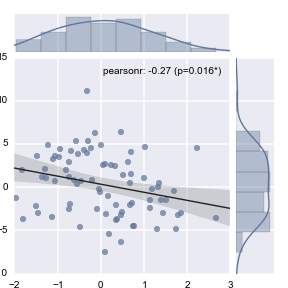
\includegraphics{sample_regression.png}
 % regression.png: 812x612 pixel, 100dpi, 20.62x15.54 cm, bb=0 0 585 441
 \label{fig:Linear Regression with Pseudo-Randomly generated Data}
 \caption{Linear regression example with Pseudo-Randomly generated data}
\end{figure}

\end{ex}

\subsubsection{Density Estimation} 
The functions h are probability densities over $Z$, and the loss function takes the form l(h;z) = l(h(z))
For instance,
\begin{equation}
 l(h(z)) = - \log h(z)
\end{equation}
is the likelihood of a point z being generated by h.
We introduce some notation - 
\begin{definition}
 We call the following the \textit{space of loss functions}
\begin{equation*}
 \mathcal{L}(\mathcal{H}) = \lbrace l(h,\cdot) : h \in \mathcal{H} \rbrace
\end{equation*}
where $\mathcal{H}$is the hypothesis.
\end{definition}
After introducing the traditional setup - we will discuss a particular kind of loss function - in a certain abstract
framework we introduce the notion of \textit{risk or generalization error} - an estimate of the expected error which can be
computed from the sample. 
\subsection{The Traditional Setup}
Consider predictors $X \in \mathcal{X}$ and responses $Y \in \mathcal{Y}$. Let \cF be a calss of functions $f:\cX \rightarrow \cY$ which take predictors as inputs. 
   Define a loss function $l: \cY \times \cY \rightarrow \mathbb{R}^{+}$ which measures the cost of making poor predictions. 
 Throughout this chapter I make the following assumption on the loss function. 
 \begin{assumption}
 $\forall f \in \cF$
 \begin{equation*}
 0 \leq l(y,y^{'}) \leq M \lt \infty
 \end{equation*}
 \end{assumption}
 Then, I can define the risk of any predictor $f \in \cF$. 
 \begin{definition}[Risk or generalization error]\label{def:risk}
 \begin{equation}
R(f):= \int l(f(X),Y) d\mathbb{P} = \mathbb{E}_{\mathbb{P}}[l(f(X),Y)], \end{equation}
where (X,Y) $\sim \mathbb{P}$
 \end{definition}
 The risk or generalization error measures the expected cost of using f to predict Y from X given a new observation. 
 Just to emphasize, the expectation is taken with respect to the distribution $\mathbb{P}$ of the test point (X,Y) which is
 independent of f; the risk is a deterministic function of f with all the randomness in the data averaged away. 
 \paragraph{} Since the true distribution \bP is unknown, so is R(f), but one can attempt to estimate it based on only the 
 observed data. Suppose that I observe a random sample $D_n = \lbrace(X_1, Y_1), \cdots,  (X_n, Y_n) \rbrace$ so that 
 $(X_i, Y_i) \stackrel{i.i.d}{\sim} \bP$, i.e. $D_n \sim \bP$. Define the \textit{training error or empirical risk} of 
 f as follows.
 \begin{dfn}[Training error or empirical risk]
 \begin{equation}\hat{R}_{n}(f):=  \dfrac{1}{n} \sum_{i=1}^{n} l(f(X_i),Y_i).
\end{equation}

 \end{dfn}
 In other words, the in-sample training error, $\hat{R}_n(f)$, is the average loss over the actual training points. 
It is easy to see that, because the training data $D_n$ and the test point (X,Y) are IID, then given some fixed function f (chosen 
independently of the sample $D_n$), 
\begin{equation}
\hat{R}_n(f) = R(f) + \gamma_n(f)
\end{equation}
where $\gamma_n(f)$ is a mean-zero noise variable that reflects how far the training sample departs from being perfectly representative of the data-generating distribution.  Here I should emphasize that $\hat{R}_n(f)$ is random enough through the training sample 
$D_n$. By the law of large numbers, for such fixed f, $\gamma_n(f) \rightarrow 0$ as $n \rightarrow \infty$, so, with enough data,
one has a good idea of how well any given function will generalize to new data.
\paragraph{} However, one is rarely interested in the performance of a single function f without adjustable parameters fixed for them in 
advance by theory. Rather, researchers are interested in a class of plausible functions \cF, possibly indexed by some possibly infinite
parameter $\theta \in \Theta$, which I refer to as a model. One fucntion (one particular parameter point) is chosen from the model class 
minimizing some criterion funciton. Maximum likelihood, Bayesian maximization \textit{a posteriori}, least squares, regularized methods, 
and empirical risk minimization (ERM) all have this flavor as do many other estimation methods. In these cases, one can define the 
empirical risk minimizer for an appropriate loss function $l$. 
\begin{definition}\label{def:Empirical_Risk_Minimizer}[Empirical Risk Minimizer]
\begin{equation}
\hat{f} := \mathrm{argmin}_{f \in \cF} \hat{R}_{n} (f) = \mathrm{argmin}_{f \in \cF} (R(f) + \gamma_n(f)).
\end{equation}\end{definition} 
It is important to note that $\hat{f}$ is random and measurable with respect to the empirical risk process $\hat{R}_n(f)$
for $f \in \cF$. Choosing a predictor $\hat{f}$ by empirical risk minimization (tuning the adjustable parameters so that $\hat{f}$
fits the training data well) conflates predicting future data well (low $R(\hat{f})$, the true risk) with exploiting the accidents and noise of the 
training data (large negative $\gamma_n(\hat{f})$, finite-sample noise). The true risk of $\hat{f}$ will generally be bigger than its in-sample risk 
precisely because I picked it to match the data well. In doing so, $\hat{f}$ ends up reproducing some of the noise in the data and therefore will not
generalize well. The difference between the true and apparent risk depends on the magnitude of the sampling fluctuations:
\begin{equation}\label{equation:3.6}
R(\hat{f}) - \hat{R}_{n}(\hat{f}) \leq \mathrm{sup}_{f\in \cF} \|\gamma_n(f)\| = \Gamma_n(\cF)
\end{equation}
In (\ref{equation:3.6}), $R(\hat{f})$ is random and measurable with respect to $\hat{f}$.
\paragraph{} The main goal of statistical learning theory is to control $\Gamma_n(\cF)$ while making minimal assumptions about the the data generating 
process - i.e. to provide bounds on over-fitting. Using more flexible models (allowing more general distributions, adding parameters, etc.) has two 
contrasting effects. On the one hand, it improves the best possible accuracy, lowering the minimum of the true risk. On the other hand, it increases 
the ability to, as it were, memorize noise for any fixed sample n. This qualitative observation - a generalization of the bias-variance trade-off from
estimation theory - can be made use-fully precise by quantifying the complexity of model classes. A typical result is a confidence bound on $\Gamma_n$ (
and hence on over-fitting), which says that with probability at least $1 - \nu$,
\begin{equation}
\Gamma_n(\cF) \leq \Theta(\Delta(\cF), n, \nu),
\end{equation} 
where $\Delta(\cdot)$ is some suitable measure of the complexity of the model $\cF$. To give specific forms of $\Theta(\cdot)$, I need to show that
for a a particular f, $R(f)$ and $\hat{R}_{n}(f)$ will be close to each other for any fixed n without knowledge of the distribution of the data. 
Furthermore, I need the complexity $\Delta(\cF)$, to claim that $R(f)$ and $\hat{R}_{n}(f)$ will be close, not only for a particular f, but
uniformly over all $f \in \cF$. Together these two results will allow me to show, despite little knowledge fo the data generating process, how bad the $
\hat{f}$ which I choose will be at forecasting future observations.
\subsection{Concentration}
The first step to controlling the difference between the empirical and expected risk is to develop concentration results for fixed functions.
We have already introduced various inequalities. McDiarmid Inequality and Hoefferding's Inequality.
These results are extremely important in Statistical learning theory, but it is beyond the scope of this thesis to go into much more detail.
In the remainder of this section, I will show how to obtain concentration for the training error around the risk for two different choices of the random
variables $Z_i$. This will lead to two different ways of controlling $\Gamma_n$ and hence the generalization error of prediction functions. 
\subsection{Contol by Counting}
Let us assume that we let $Z_i$ be the loss of the $i^{th}$ training point for some fixed function f. 
Then by Hoeffding's inequality we get the following remarkable result
\begin{equation}
\mathbb{P}^n\left(\|R(f) - \hat{R}_{n}(f) \| \geq \epsilon \right) \leq 2 \exp\lbrace - \dfrac{2n\epsilon^{2}}{M^2}\rbrace
\end{equation}
This result is quite powerful, it says that the probability of observing data which will result in a training error much different from the expected 
risk goes to zero exponentially with the size of the training set. The only assumption necessary was $0 \leq l(y,y^{'}) \leq M \lt \infty$.
\subsection{Capacity}
\label{sec:capacity}

For ``small'' models, we can just count the number of functions in the class
and take the union bound. Suppose that $\F = \{f_1,\ldots,f_N\}$. Then we have
\begin{align}
  \P\left( \sup_{1\leq i \leq N} |R(f_i) - \hat{R}_n(f_i)| > \epsilon
  \right)& \leq \sum_{i=1}^N \P\left(  |R(f_i) - \hat{R}_n(f_i)| > \epsilon
  \right) \\ &\leq N\exp\left\{ - \frac{2n\epsilon^2}{K}\right\},
  \label{eq:union-bound}
\end{align}
by Theorem \ref{thm:hoeffding}. Most interesting models are not small in this
sense, but similar results hold when model size is measured
appropriately.

There are a number of measures for the size or capacity of a model.
Algorithmic stability
\cite{KS_1998,bousquet2002stability} quantifies
the sensitivity of the chosen function to small perturbations to the data.
Similarly, maximal discrepancy \cite{vapnik2000nature} asks how different the
predictions could be if two functions are chosen using two separate data sets.
A more direct, functional-analytic approach partitions $\F$ into equivalence
classes under some metric, leading to covering numbers
\cite{Pollard1990}.  Rademacher complexity
\cite{Bartlett} directly describes a model's ability to fit
random noise. We focus on a measure which is both intuitive and powerful:
Vapnik-Chervonenkis (VC) dimension \cite{vapnik2000nature}.

VC dimension starts as an idea about collections of sets.
\begin{definition}
  Let $\mathbb{U}$ be some (infinite) set and $S$ a finite subset of
  $\mathbb{U}$. Let $\mathcal{C}$ be a family of subsets of $\mathbb{U}$. We
  say that $\mathcal{C}$ \emph{shatters} $S$ if for every $S' \subseteq S$,
  $\exists C \in\mathcal{C}$ such that $S' = S \cap C$.
\end{definition}
Essentially, $\mathcal{C}$ can shatter a set $S$ if it can pick out every
subset of points in $S$. This says that the collection $\mathcal{C}$ is very
complicated or flexible. The cardinality of the largest set $S$ that can be
shattered by $\mathcal{C}$ is the latter's VC dimension.
\begin{definition}
  [VC dimension]
  The \emph{Vapnik-Chervonenkis (VC) dimension} of a collection
  $\mathcal{C}$ of subsets of $\mathbb{U}$ is
  \begin{equation}
    \vcd(\mathcal{C}) := \sup \{ |S| : S\subseteq \mathbb{U}\mbox{ and
      $S$ is shattered by
    } \mathcal{C} \}.
  \end{equation}
\end{definition}
To see why this is a ``dimension'', we need one more notion.
\begin{definition}
  [Growth function] The \emph{growth function} $G(\mathcal{C},n)$ of a
  collection $\mathcal{C}$ of subsets of $\mathbb{U}$ is the maximum
  number of
  subsets which can be formed by intersecting a set $S \subset \mathbb{U}$ of
  cardinality $n$ with $\mathcal{C}$,
  \begin{equation}
    G(n,\mathcal{C}) := \sup_{S\subset U~:~ |S|=n}{|S\wedge \mathcal{C}|}
  \end{equation}
\end{definition}
The growth function counts how many {\em effectively} distinct sets the
collection contains, when we can only observe what is going on at $n$ points,
not all of $\mathbb{U}$.  If $n \leq \vcd(\mathcal{C})$, then from the definitions
$G(n,\mathcal{C}) = 2^n$, If the VC dimension is finite, however, and $n >
\vcd(\mathcal{C})$, then $G(n,\mathcal{C}) < 2^n$, and in fact it can be shown
\cite{VapnikChervonenkis1971} that
\begin{equation}
  G(n,\mathcal{C}) \leq
  (n+1)^{\vcd(\mathcal{C})}.
\end{equation}
This polynomial
growth of capacity with $n$ is why $\vcd$ is a ``dimension''.  
% The bound on the
% growth function will recur several times in our results, so we define
% \begin{equation}
% GF(n,h) := (n+1)^h
% \end{equation}

Using VC dimension to measure the capacity of function classes is
straightforward.  Define the indicator function $\indicator_A(x)$ to take the
value 1 if $x\in A$ and 0 otherwise. Suppose that $f\in\F$,
$f:\mathbb{U}\rightarrow\R$. Each $f$ corresponds to the set
\begin{equation}
C_f = \{ (u,a) : \indicator_{(0,\infty)}(f(u)-b)=1,\ \ u\in\mathbb{U},\ \ b\in\R\},
\end{equation}
so $\F$ corresponds to the class $\mathcal{C}_\F := \{ C_f : f \in \F\}$.
Essentially, the growth function $G(n,\vcd(\F))$ counts the effective number of
functions in $\F$, i.e., how many can be told apart using only $n$
observations.  When $\vcd(\F) < \infty$, this number grows only polynomially
with $n$.  This observation lets us control the risk over the entire model,
providing one of the pillars of statistical learning theory.

\begin{theorem}
  [\cite{VapnikChervonenkis1971}]
  \label{thm:vapnik}
  Suppose that $\vcd(\F)< \infty$ and $0\leq\ell(y,y')\leq K <
  \infty$. Then, 
  \begin{equation}
    \label{eq:vcbound}
    \P \left(\sup_{f\in\F} |R(f) - \hat{R}_n(f)| > \epsilon\right)
    \leq 4(2n+1)^{\vcd(\F)} \exp \left\{ - \frac{n\epsilon^2}{K^2_1} \right\} ~,
  \end{equation}
  where $K_1$ depends only on $K$ and not $n$ or $\F$.
\end{theorem}
The proof of this theorem has a similar flavor to the union bound argument
given in \ref{eq:union-bound}.

This theorem has as an immediate corollary a bound for the out-of-sample
risk. Since $\sup_{f\in {\cal F}}$ is inside the probability statement in
\ref{eq:vcbound}, it applies to both pre-specified and to data-dependent
functions, including any $\widehat{f}$ chosen by fitting a model or minimizing
empirical risk. 
\begin{corollary}
  \label{cor:vapnik}
  When \ref{thm:vapnik} applies, for any $\eta>0$ and any $f \in \F$, with probability at least $1-\eta$,
  \begin{equation}
  R(f) \leq \widehat{R}_n(f) + K_1\sqrt{\frac{\vcd(\F)\log(2n+1) +
      \log 4/\eta}{n}}.
  \end{equation}
\end{corollary}
The factor $K_1$ can be calculated explicitly but is unilluminating and we will not
need it.  Conceptually, the right-hand side of this inequality resembles
standard model selection criteria, like AIC or BIC, with in-sample fit plus a
penalty term which goes to zero as $n\rightarrow\infty$. Here however, the
bound holds with high probability despite lack of knowledge of $\P$ and it has
nothing to do with asymptotic convergence: it holds for each $n$.  It does
however hold {\em only} with high $\P$ probability, not always.

\begin{figure}[h]
 \centering
 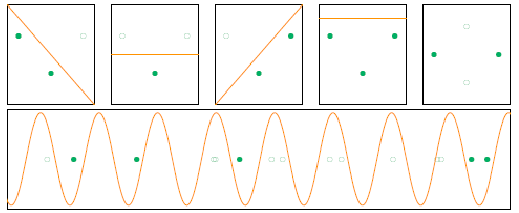
\includegraphics[bb=0 0 389 160]{ShatterSetpicture.png}
 % ShatterSetpicture.png: 519x213 pixel, 96dpi, 13.73x5.64 cm, bb=0 0 389 160
 \caption{Illustration of VC dimension for some function classes.}
 \label{fig:Illustration of VC Dimensions}
\end{figure}

VC dimension is well understood for some function classes. For instance, if
$\F=\{\mathbf{x}\mapsto \bs{\gamma}\cdot\mathbf{x} : \bs{\gamma} \in \R^p\}$
then $\vcd(\F)=p+1$, i.e. it is the number of free parameters in a linear
regression plus 1.  VC dimension does not always have such a nice relation to
the number of free parameters however; the classic example is the model
$\F=\{x\mapsto \sin(\omega x) : \omega \in \R\}$, which has only one free
parameter, but $\vcd(\F)=\infty$.\footnote{This result follows if we can show
  that for any positive integer $J$ and any binary sequence $(r_1,\ldots,r_J)$,
  there exists a vector $(x_1,\ldots,x_J)$ such that
  $\indicator_{[0,1]}(\sin(\omega x_i))=r_i$. If we choose $x_i=2\pi 10^{-i}$,
  then one can show that taking $\omega=\frac{1}{2}\left(\sum_{i=1}^J
    (1-r_i)10^i +1\right)$ solves the system of equations.} These examples are illustrated in
\ref{fig:Illustration of VC Dimensions}. At the
same time, there are model classes (support vector machines) which may
have infinitely many parameters but finite VC dimension. 
\cite{CristianiniShawe-Taylor2000}. This illustrates a further
difference between the statistical learning approach and the usual information
criteria, which are based on parameter-counting.

The concentration results in \ref{thm:vapnik} and \ref{cor:vapnik} work
well for independent data. The first shows how quickly averages concentrate around
their expectations: exponentially fast in the size of the data.  The second
result generalizes the first from a single function to entire function classes.
Both results, as stated, depend critically on the independence of the random
variables.  For time series, we must be able to handle dependent data.  In
particular, because time-series data are dependent, the length $n$ of
a sample
path $Y_1,\ldots,Y_n$ exaggerates how much information it contains.  Knowing
the past allows forecasters to predict future data (at least to some degree),
so actually observing those future data points gives less information about the
underlying process than in the IID case. Thus, while in \ref{thm:hoeffding}
the probability of large discrepancies between empirical means and their
expectations decreases exponentially in $n$, in the dependent case, the
effective sample size may be much less than $n$ resulting in looser bounds. 
\section{Rademacher Processes}\label{sec:Rademacher}
We introduce very quickly some remarks from Rademacher Processes,
and some key techniques. This is merely to show the 

A key technique in the theory of empirical processes is \textit{Rademacher symmetrization}. 
This was first introduced into empirical processes in a classical paper by Gine \cite{Gine1984}
so we'll show how this applies in the context of Talagrand's inequality\cite{Talagrand95,TalagrandInequality}. 
\paragraph{} Let $\epsilon_i,i=1,\cdots,n,$ be i.i.d Rademacher random signs (taking values -1,1 with probability 1/2), independent of the $X'_{i}s$, defined on a large product probability space with product probability Pr, denote the joint expectation by E, and the $E_{\epsilon}$ and $E_{X}$ the corresponding expectations w.r.t the $\epsilon_i 's$ $X'_{i}s$,
respectively. The following symmetrization inequality holds for random variables in arbitrary normed spaces, but we state it for the suprenum norm relevant in empirical process theory: For $\mathcal{F}$ a class of functions on $(S,\mathcal{A})$, define $\|
H\|_{\mathcal{F}} = \mathrm{sup}_{f \in \mathcal{F}} |H(f)|$.

\begin{lem}
Let $\mathcal{F}$ be a uniformly bounded P-centered class of functions defined on a measurable space $(S,\mathcal{A})$. Let 
$\epsilon_{i}$ be i.i.d. Rademachers as above, and let $a_i, i = 1,\cdots,n$ be any sequence of real numbers. Then
\begin{equation}
\dfrac{1}{2}E \|\sum_{i=1}^{n} \epsilon_{i} f(X_{i})\|_{\mathcal{F}} \leq 
E \|\sum_{i=1}^{n} f(X_i)\|_{\mathcal{F}} \leq \|\sum_{i=1}^{n} \epsilon_{i}(f(X_i)+a_{i})\|_{\mathcal{F}}
\end{equation}
\end{lem}
\begin{proof}
Let us assume for simplictly that $\mathcal{F}$ is countable (so
that we can neglect measurability problems). Since $E_{X}f(X_{i}) = 0$ for every $f,i,$ the first inequality follows from
\begin{eqnarray*}
E \|\sum_{i=1}^{n} \epsilon_{i}(f(X_i)\|_{\mathcal{F}}
= E_{\epsilon} E_{X} \leq E_{\epsilon} E_{X} \|\sum_{i: \epsilon_{i} = -1}f(X_{i}) + E_{X} \sum_{i: \epsilon_{i} =1}f(X_{i})\|_{\mathcal{F}}
 \\ + E_{\epsilon} E_{X} \|\sum_{i: \epsilon_{i} = 1}f(X_{i}) + E_{X} \sum_{i: \epsilon_{i} = -1}f(X_{i})\|_{\mathcal{F}}
 \leq 2E \|\sum_{i=1}^{n} f(X_{i})\|_{\mathcal{F}}
\end{eqnarray*}
where in the last inequality we have used Jensen's inequality and convexity of the norm. To prove the second inequality, let 
$X_{n+i}, i =1,\cdots,n$ be an independent copy of $X_1, \cdots, 
X_n$. Then proceeding as above,
$E\|\sum_{i=1}^{n} f(X_{i})\|_{\mathcal{F}} = E \|\sum_{i=1}^{n}(f(X_{i}) - E f(X_{n+i})\|_{\mathcal{F}} \leq E \|\sum_{i=1}^{n}(f(X_{i} + a_i) - \sum_{i=1}^{n}(f(X_{n+i}+a_i)\|_{\mathcal{F}}$

which clearly equals
\begin{equation*}
E_{\epsilon}E_X \|\sum_{i: \epsilon_{i}=1} \epsilon_i (f(X_i) + a_i - f(X_{n+i}) -a_{i}
- \sum_{i: \epsilon_{i}=-1} \epsilon_i (f(X_i) + a_i - f(X_{n+i}) -a_{i}\|_{\mathcal{F}}
\end{equation*}
Now Pr being a product probability measure with identical coordinates, it is invariant by permutations of the coordinates, so that we may exchange $f(X_i)$ and $f(X_{n+i})$ for the i's where
$\epsilon_i = -1$ in the last expectation. This gives that the quantity in the last equation equals 
\begin{equation*}
 E_{\epsilon} E_X \|\sum_{i=1}^{n} \epsilon_i(f(X_i)) + a_{i} - f(X_{n+i}) - a_{i})\|_{\mathcal{F}}\leq 2E \|\sum_{i=1}^{n} \epsilon_i(f(X_{i}) +a_i)\|_{\mathcal{F}}
\end{equation*} which completes the proof.
\end{proof}
This simple but very useful result says that we can always compare the size of the expectation of the 
supremum of an empirical process to a symmetrized process. The idea usual is that the symmetrized
\textit{Rademacher} process has conditional on the $X_i's$ a very simple structure. 
One can then derive results of the Rademacher proecess and integrate the results over the distribution of the  $X_i's$
Rademacher averages are quantities that play an important role in empirical process
theory\cite{dudley1999uniform} and in
the theory of Banach spaces\cite{Ledoux}.
We shall not consider more about Rademacher averages in this paper and suggest \cite{SLT_Lugosi_Bocheron, Bartlett}
as reading material. 
The concentration results in \ref{thm:vapnik} and \ref{cor:vapnik} work
well for independent data. The first shows how quickly averages concentrate around
their expectations: exponentially fast in the size of the data.  The second
result generalizes the first from a single function to entire function classes.
Both results, as stated, depend critically on the independence of the random
variables.  For time series, we must be able to handle dependent data.  In
particular, because time-series data are dependent, the length $n$ of
a sample
path $Y_1,\ldots,Y_n$ exaggerates how much information it contains.  Knowing
the past allows forecasters to predict future data (at least to some degree),
so actually observing those future data points gives less information about the
underlying process than in the IID case. Thus, while in \ref{thm:hoeffding}
the probability of large discrepancies between empirical means and their
expectations decreases exponentially in $n$, in the dependent case, the
effective sample size may be much less than $n$ resulting in looser bounds.


\section{Time series}
\label{sec:dependence}
Before we proceed it is worth including a definition of \emph{time series}
and a visual example.
\begin{definition}
 A time series is a collection of observations 
of well-defined data items obtained through repeated measurements over time.
\end{definition}
We include an example of time series data - plotted using freely available USDA data on meat production.\footnote{
This data is included in the Pandas Python library\cite{Pandas}
 or at \url{http://www.ers.usda.gov/data-products/livestock-meat-domestic-data.aspx}}
\begin{figure}[ht]
 \centering
 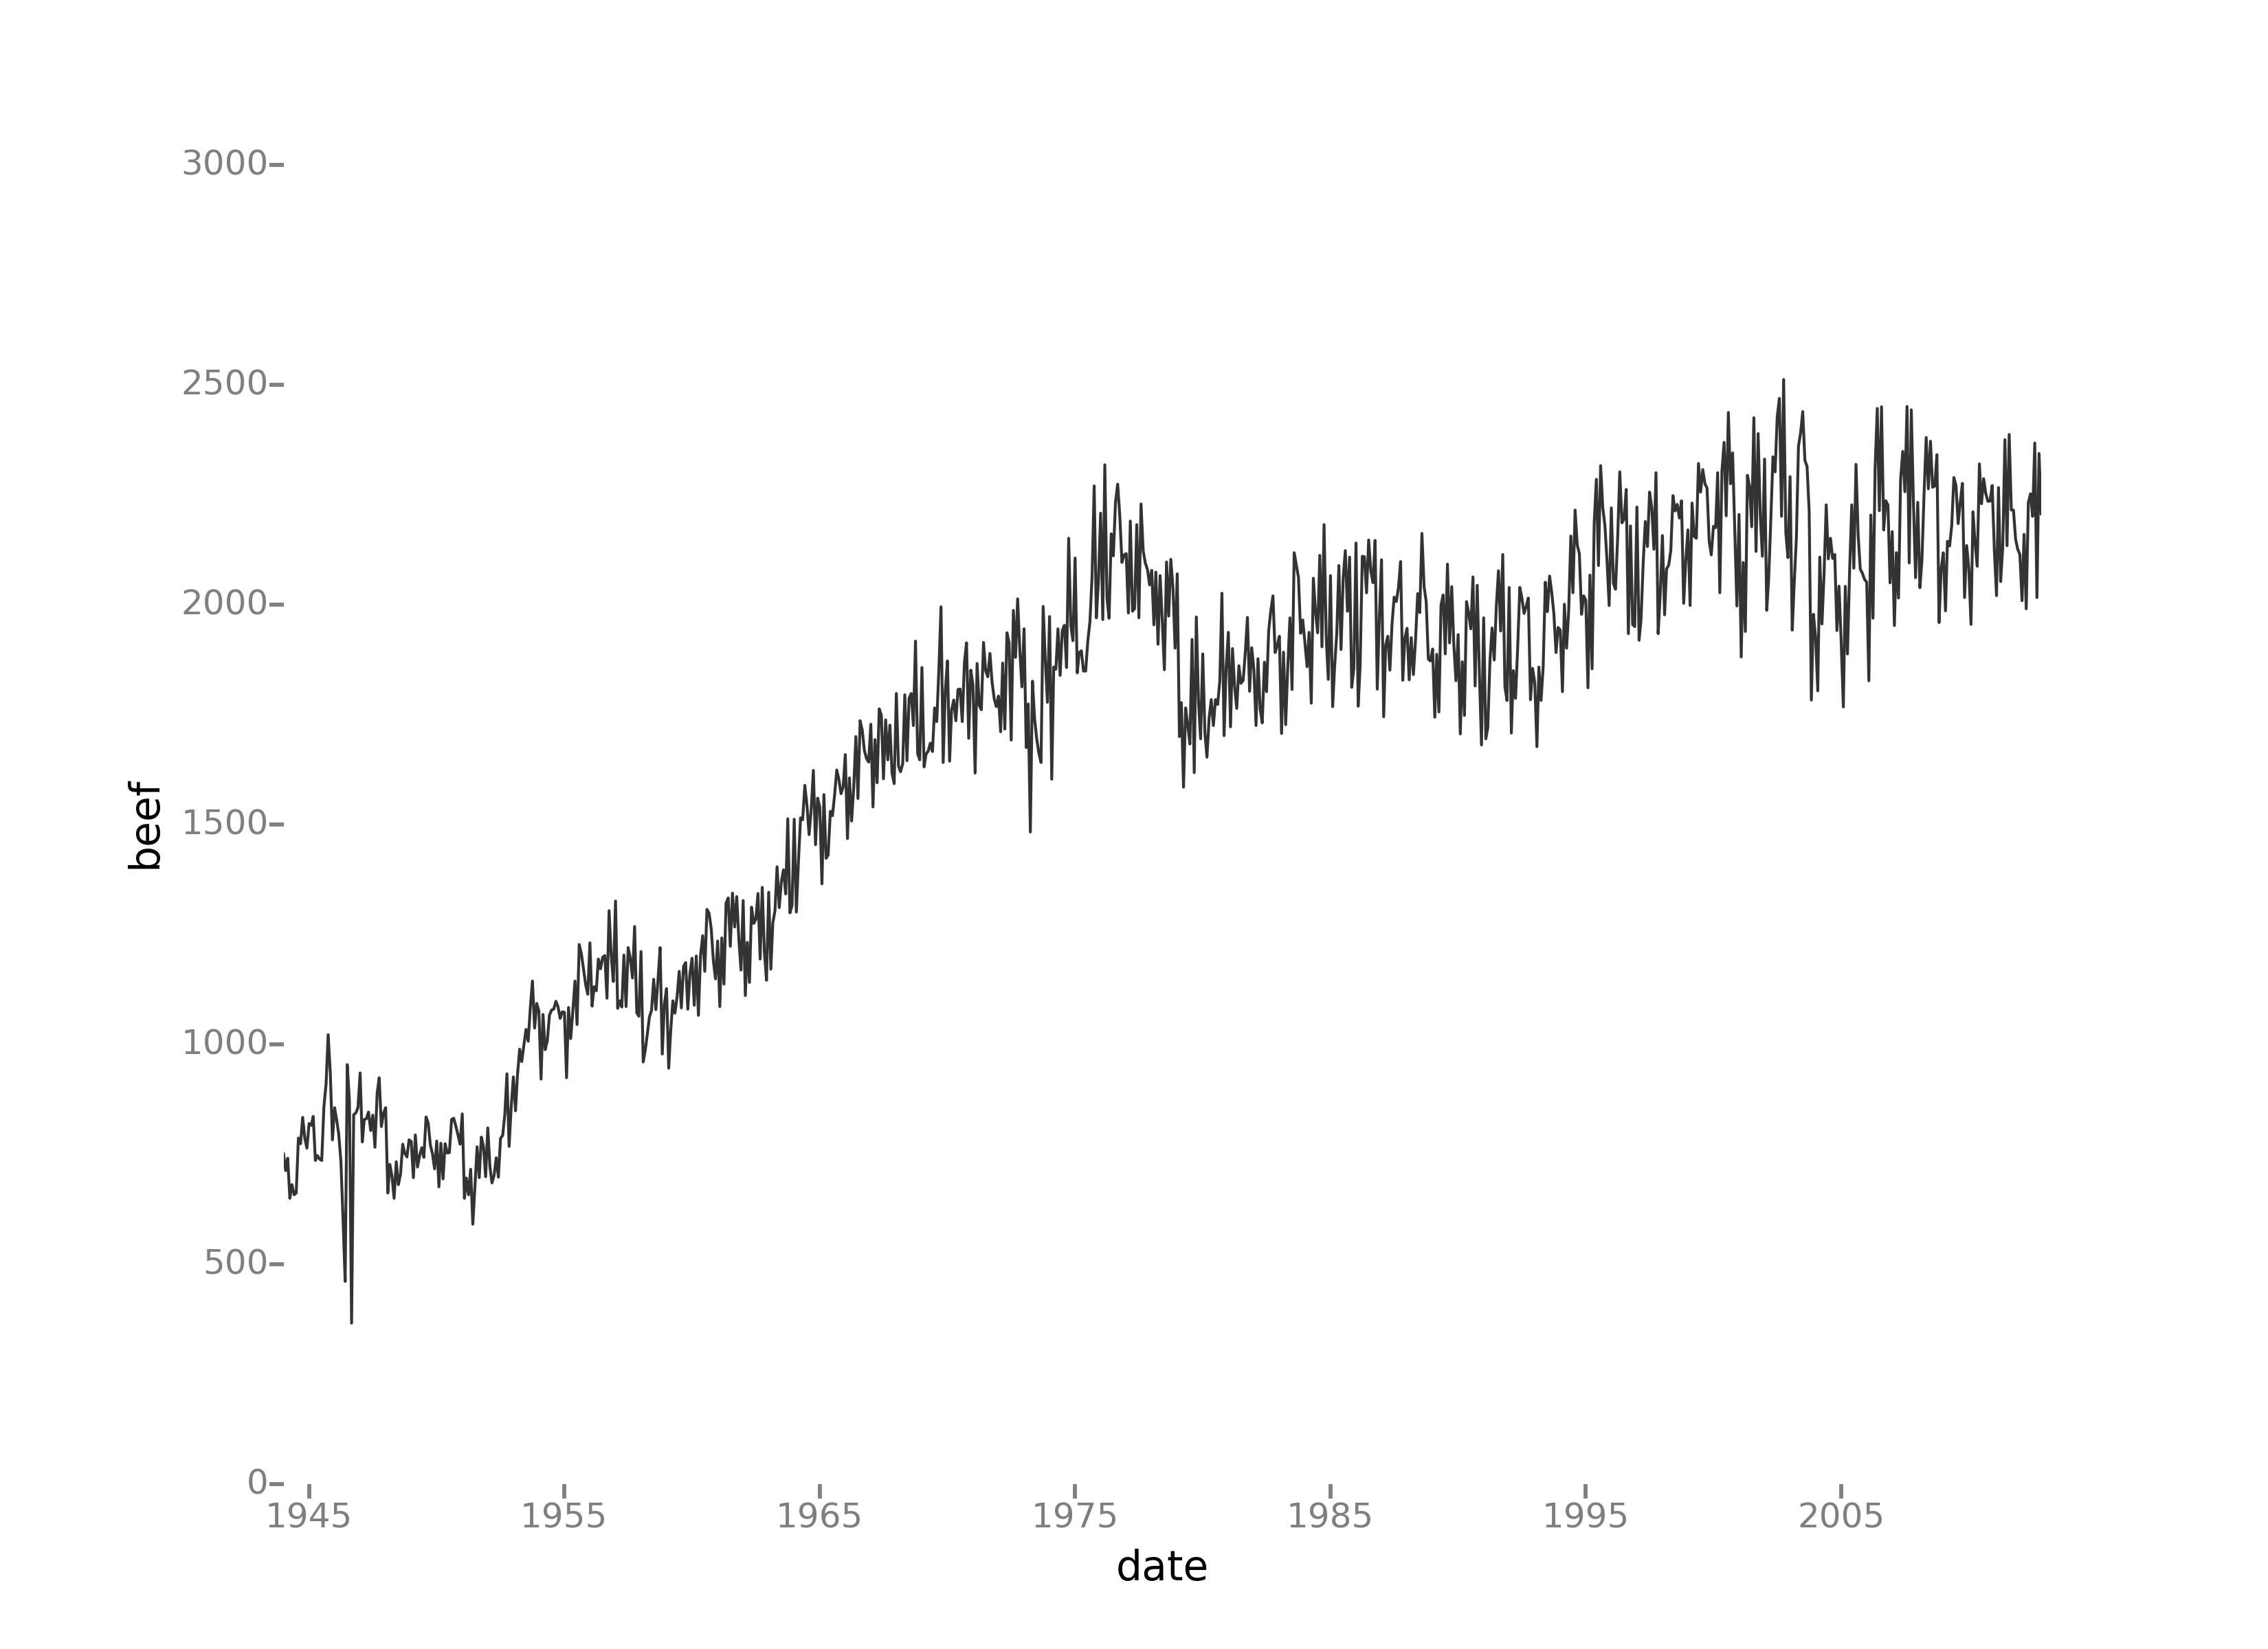
\includegraphics[bb=0 0 792 576,scale=0.5]{timeseries.png}
 % timeseries.png: 3300x2400 pixel, 300dpi, 27.94x20.32 cm, bb=0 0 792 576
 \caption{Time Series example showing the changes in Beef consumption over the 20th Century in the US}
 \label{fig:Time Series of USDA Meat Data}
\end{figure}


In moving from the IID setting to time series forecasting, we need a number of
modifications to our initial setup.  Rather than observing input/output pairs
$(Y_i,X_i)$, we observe a single sequence of random variables
$\Yin:=(Y_1,\ldots,Y_n)$ where each $Y_i$ takes values in
$\R^p$.\footnote{We can easily generalize this to arbitrary
  measurable spaces.}  We are interested in using functions which
take past observations as inputs and predict future values of the process.
Specifically, given data from time 1 to time $n$, we wish to predict time
$n+1$.


While we no longer presume IID data, we still need to restrict the sort of dependent
process we work with.  We first remind the reader of the notion of (strict or
strong) stationarity.
\begin{definition}[Stationarity]\label{def:stationary}
  A random sequence $\Yinf$ is stationary when all its finite-dimensional
  distributions are time-invariant: for all $t$ and all non-negative integers
  $i$ and $j$, the random vectors $\Yij{t}{t+i}$ and $\Yij{t+j}{t+i+j}$ have
  the same distribution.
\end{definition}
Stationarity does not imply that the random variables $Y_t$ are independent
across time $t$, only that the unconditional distribution of $Y_t$ is constant
in time.  We limit ourselves not just to stationary processes, but also to ones
in which widely-separated observations are asymptotically independent.  Without
this restriction, convergence of the training error to the expected risk could
occur arbitrarily slowly, and finite-sample bounds may not exist.\footnote{In
  fact, \cite{AdamsNobel2010} demonstrate that for ergodic processes, finite
  VC dimension is enough to give consistency, but not rates.}  The next
definition describes the sort of serial dependence which we entertain.
\begin{definition}[$\beta$-Mixing]
  \label{defn:beta-mix}
  Consider a stationary random sequence $\Yinf$ defined on
  a probability space $(\Omega, \Sigma, \Pinf)$. Let $\Sij{i}{j}=\sigma(\Yij{i}{j})$ be the $\sigma$-field of events
  generated by the appropriate collection of random variables.  Let $\P_0$ be
  the restriction of $\Pinf$ to $\Sij{-\infty}{0}$, $\P_{a}$ be the
  restriction of $\Pinf$ to $\Sij{a}{\infty}$, and $\P_{0\otimes a}$ be the
  restriction of $\Pinf$ to
  $\sigma(\Yij{\infty}{0},\Yij{a}{\infty})$.  The {\em
    coefficient of absolute regularity}, or {\em $\beta$-mixing coefficient},
  $\beta_a$, is given by
\begin{equation}
  \label{eq:three}
  \beta_a := ||\P_0 \times \P_{a} - \P_{0 \otimes
    a}||_{TV}, 
\end{equation}
where $|| \cdot ||_{TV}$ is the total variation norm. A stochastic process is
{\em absolutely regular}, or {\em $\beta$-mixing}, if $\beta_a \rightarrow 0$
as $a\rightarrow\infty$.
\end{definition}
This is only one of many equivalent characterizations of $\beta$-mixing (see
\cite{Bradley2005} for others).  This definition makes clear that a process is
$\beta$-mixing if the joint probability of events which are widely separated in
time approaches the product of the individual probabilities, i.e., that $\Yinf$
is asymptotically independent.  Many common time series models are known to be
$\beta$-mixing, and the rates of decay are known up to constant factors which
are functions of the true parameters of the process.  Among the processes for
which such results are known are ARMA models \cite{Mokkadem1988}, GARCH models
\cite{CarrascoChen2002}, and certain Markov processes --- see
\cite{doukhan1994mixing} for an overview.  Additionally, functions of $\beta$-mixing
processes are $\beta$-mixing, so if $\Pinf$ could be specified by a dynamic
factor model or DSGE or VAR, the observed data would satisfy this condition.

Knowing $\beta_a$ would let us determine the effective sample size of time
series $\Yin$.  In effect, having $n$ dependent-but-mixing data points is like
having $\mu<n$ independent ones.  Once we determine the correct $\mu$, we can
(as we will now show) use concentration results for IID data like those in
\ref{thm:hoeffding} and \ref{thm:vapnik} with small corrections.

\section{Risk bounds}
\label{sec:risk-bounds}

With the relevant background in place, we can put the pieces together to derive
our results. We use $\beta$-mixing to find out how much information is in the
data and VC dimension to measure the capacity of the state-space model's
prediction functions. The result is a bound on the generalization error of the
chosen function $\hat{f}$.  After slightly modifying the definition of ``risk''
to fit the time-series forecasting scenario, and stating necessary technical
assumptions, we derive risk bounds for wide classes of economic forecasting
models.



\subsection{Setup and assumptions}
\label{sec:setup-assumptions}

We observe a finite subsequence of random vectors $\Yin$ from a process $\Yinf$
defined on a probability space $(\Omega, \Sigma, \P_\infty)$, with $Y_i \in
\R^p$. We make the following assumption on the process.
\begin{assumption}
  \label{ass:A}
  $\P_\infty$ is a stationary, $\beta$-mixing process with mixing
  coefficients\footnote{In order to apply the results, one must either
    know $\beta_a$ for some $a$ or be able to estimate it with
    sufficient precision and accuracy. \cite{McDonald_TimeSeries} shows how to estimate the
    mixing coefficients non-parametrically, based on a single sample from the
    process.} $\beta_a$, $\forall a>0$.
\end{assumption}

Under stationarity, the marginal distribution of $Y_t$ is the same for all $t$.
We deal mainly with the joint distribution of $\Yini$, where we observe the
first $n$ observations and try predicting $Y_{n+1}$.  For the rest of this
paper, we will call this joint distribution $\P$. Our results extend to
predicting more than one step ahead, but the notation becomes cumbersome.

We must define generalization error and training error slightly differently for
time series than in the IID setting.  Using the same notion of loss functions
as before, we consider prediction functions $f : \R^{n\times p} \rightarrow
\R^p$
\begin{definition}
  [Time series risk]
  \begin{equation}
  R_n(f) := \E \Big[ \mnorm{ Y_{n+1} - f(\Yin)} \Big].
  \end{equation}
\end{definition}
The expectation is taken with respect to the joint distribution $\P$ and
therefore depends on $n$.  The function $f$ may use some or all of the past to
generate predictions.  A function using only the most recent $d$ observations
as inputs will be said to have \emph{fixed memory} of length $d$. Other
functions have \emph{growing memory}, i.e., $f$ may use all the previous data
to predict the next data point.  This incongruity makes the notation
for time series training error somewhat problematic.

We will define the
training error with a subscript $i\in\mathbb{N}$ on $f$ within the summation.
Strictly speaking, there is only one function $f$ which we are using
to make forecasts. In typical fixed memory settings --- standard VAR
forecasting models and so on --- $f_i=f_j=f$ for all $i,j \in \mathbb{N}$. But
for models with growing memory, a fixed forecasting method ---
an ARMA model, DSGE,\footnote{A DSGE is a nonlinear system of expectational
  difference equations, so estimating the parameters is nontrivial.  Likelihood
  methods typically work by finding a linear approximation using Taylor
  expansions and the Kalman filter, though increasingly complex nonlinear
  methods are now intensely studied.  See for instance
  \cite{DeJongDave2007} or
  \cite{DejongDharmarajan2009}} or linear state-space model --- will use all of
the past to make predictions, so the dimension of the domain changes
with $i$. We write the risk of $f$ as a single function, because, once
we parameterize a forecasting method, an entire sequence of
forecasting functions $f_1,f_2,\ldots$ is determined. 
\begin{definition}
  [Time series training error]
  \begin{equation}
  \hat{R}_n(f) := \frac{1}{n-d-1} \sum_{i=d}^{n-1} \mnorm{Y_{i+1} - f_i(\Yij{1}{i})}.
  \end{equation}
\end{definition}
% \begin{definition}
%   [Time series training error with growing memory (at least $d$)]
%   \begin{equation}
%   \widetilde{R}_n(f) := \frac{1}{n-d-1} \sum_{i=d}^{n-1} \mnorm{Y_{i+1} - f(\Yij{1}{i})}.
%   \end{equation}
% \end{definition}
In order to make
use of this single definition of training error, we let $d \geq 0$.
In fixed memory cases --- say an AR(2) --- $d$ has an obvious
meaning, while with growing memory, $d=0$ is allowed.

To control the generalization error for time series forecasting, we make one
final assumption, about the possible magnitude of the losses.  Specifically, we
weaken the bounded loss assumption we used in \ref{sec:SLT} to
allow for unbounded loss as long as we retain some control on moments of the
loss.
\begin{assumption}
  \label{ass:B}
  Assume that for all $f \in \F$
  \begin{equation}
 Q_n(f) := \sqrt{\E_\P\Big[\mnorm{Y_{n+1}-f(\Yin)}^2
   \Big]}\leq M < \infty.
  \end{equation}
\end{assumption}
\ref{ass:B} is still quite general, allowing even some heavy tailed
distributions.

\subsection{Fixed memory}
\label{sec:fixed-memory}


We can now state our results giving finite sample risk bounds for the problem
of time series forecasting.  We will only consider the fixed-memory situation, even though most DSGE\cite{DeJongDave2007}
models having growing memory. 

\begin{theorem}
  \label{thm:bound1}
  Suppose that \ref{ass:A} and \ref{ass:B} hold, that the model class
  $\F$ has a fixed memory length $d<n$, and that we have a sample
  $\mathbf{Y}_1^n$. Let $\mu$ and $a$ be integers such that $2\mu a+d\leq
  n$. Then, for all $\epsilon>0$,
  \begin{align}
    \label{eq:bound1}
      \lefteqn{\P\left( \sup_{f \in \F} \frac{R_n(f) - \widehat{R}_n(f)}{Q_n(f)}
        > \epsilon \right)}\\ &\leq 8 (2\mu+1)^{\vcd(\F)}\exp\left\{ -
        \frac{\mu\exp\left(W\left(-\frac{2\epsilon^2}{e^4}\right)+4\right)}{4}
      \right\} + 2\mu\beta_{a-d},\nonumber 
    \end{align}
    where $W(\cdot)$ is the Lambert W function.
\end{theorem}


The implications of this theorem are considerable. Given a finite
sample of length
$n$, we can say that with high probability, future prediction
errors will not be much larger than our observed training errors. It makes no
difference whether the model is correctly specified. This stands in stark
contrast to model selection tools like AIC or BIC which appeal to
asymptotics. Moreover, given a model class $\F$, we can say exactly how much
data we need to have good control of the prediction risk. As the effective data
size increases, the training error is a better and better estimate of the
generalization error, uniformly over all of $\F$.

The Lambert W function in the exponential term deserves some explanation. The Lambert W
function is defined as the  inverse of $f(w) = w\exp{w}$
(cf. \cite{CorlessGonnet1996}). A strictly, but only slightly, worse
bound can be achieved by noting that
\begin{equation}
\label{eq:worsebound}
\exp\left(W\left(-\frac{2\epsilon^2}{e^4}\right)+4\right)\leq \frac{\epsilon^{8/3}}{4^{2/3}}
\end{equation}
for all $\epsilon\in [0,1]$.

The difference between expected and empirical risk is only interesting
when $R_n(f)$ exceeds $\widehat{R}_n(f)$.  Due to the supremum, events where the training error
exceeds the expected risk are irrelevant. Therefore, we are only concerned with
$0 \leq \hat{R}_n(f) \leq R_n(f)$. Of course, as discussed in
\ref{sec:SLT}, for most estimation
procedures, $f$ is chosen to make $\widehat{R}_n(f)$ as small as
possible.

One way to understand this theorem is to visualize the tradeoff between
confidence $\epsilon$ and effective data $\mu$.  Consider, by
way of illustration, what happens when $\vcd(\F) = 1$, $\beta_a =
0$, and $M=1$. Then \ref{thm:bound1} and \ref{eq:worsebound} become
\begin{equation}
  \P\left( \sup_{f \in \F} R_n(f) - \widehat{R}_n(f)
    > \epsilon \right) \leq 8 \exp\left\{\log (2\mu+1) -
    \frac{\mu\epsilon^{8/3}}{4^{5/3}} \right\} 
\end{equation}
Our goal is to minimize $\epsilon$, thereby ensuring that the relative
difference between the expected risk and the training risk is small. At the
same time we want to minimize the right side of the bound so that the
probability of ``bad'' outcomes --- samples where the difference in risks
exceeds $\epsilon$ --- is small. Of course we want to do this with as little
data as possible, but the smaller we take $\epsilon$, the larger we must take
$\mu$ to compensate.  We depict this tradeoff in \ref{fig:risk}.


The figure is structured so that movement toward the origin is preferable.  We
have tighter control on the difference in risks with less data. But moving in
that direction leads to an increased probability of the bad event --- that the
difference in risks exceeds $\epsilon$. The bound becomes trivial below the
solid black line (the bad event occurs with probability no larger than
one). The desire for the bad event to occur with low probability forces the
decision boundary to the upper right.

Another way to interpret the plot is as a set of indifference
curves. Anywhere in the same color region is equally desirable in the
sense that the probability of equally bad events is the same. So if we had a
budget constraint trading $\epsilon$ and data (i.e. a line with negative
slope), we could optimize within the budget set to find the lowest
probability allowable.  
\begin{figure}[t!]
  \centering
  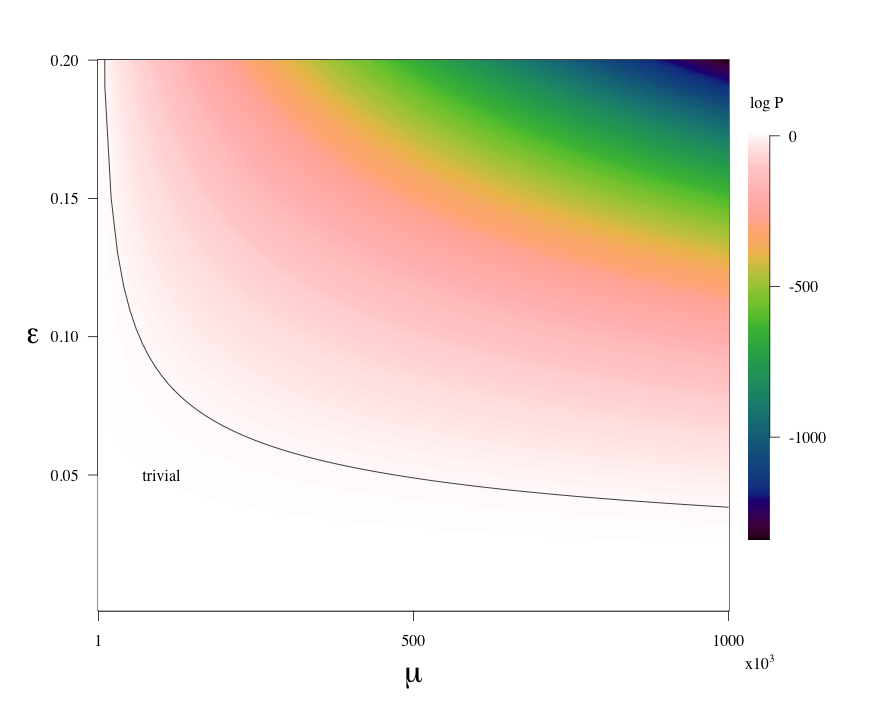
\includegraphics[width=5in]{smoothplot.png}
  \caption{Visualizing the tradeoff between confidence ($\epsilon$, $y$-axis)
    and effective data ($\mu$, $x$-axis). The black curve indicates the region
    where the bound becomes trivial. Below this line, the probability is
    bounded by 1. Darker colors indicate lower probability of the ``bad'' event
    --- that the difference in risks exceeds $\epsilon$. The colors correspond
    to the natural logarithm of the bound on this probability.}
  \label{fig:risk}
\end{figure}


Before we prove \ref{thm:bound1}, we will state a corollary which puts the
same result in a form that is sometimes easier to use.

\begin{corollary}
  \label{cor:bound1}
  Under the conditions of \ref{thm:bound1}, for any $f \in \F$, the
  following bound holds with probability at least $1-\eta$, for all
  $\eta>2\mu\beta_{a-d}$:
  \begin{equation}
    \label{eq:bound-with-known-vc}
    R_n(f) \leq \widehat{R}_n(f) +M
    \sqrt{ \frac{ \mathcal{E}(4-\log \mathcal{E})}{2}},
  \end{equation}
  with
  \begin{equation}
    \label{eq:bound-magnitude}
    \mathcal{E} = \frac{4\vcd(\F)\log(2\mu+1) + \log 8/\eta'}{\mu},
  \end{equation}
  and $\eta'=\eta-2\mu\beta_{a-d}$.
\end{corollary}
We now prove both \ref{thm:bound1} and \ref{cor:bound1} to provide the
reader with some intuition for the types of arguments necessary.  We defer
proof of the remainder of the theorems in this section to the appendix.
\begin{proof}[Proof of \ref{thm:bound1} and \ref{cor:bound1}]
  The first step is to move from the actual sample size $n$ to the effective
  sample size $\mu$ which depends on the $\beta$-mixing behavior.  Let $a$ and
  $\mu$ be non-negative integers such that $2a\mu + d \leq n$. Now divide
  $\mathbf{Y}_1^{n}$ into $2\mu$ blocks, each of length $a$, ignoring
  the remainder. Identify the
  blocks as follows:
  \begin{align}
    U_j &= \{Y_i: 2(j-1)a + 1 \leq i \leq (2j-1)a\},\\
    V_j &= \{Y_i : (2j-1)a + 1 \leq i \leq 2ja\}.
  \end{align}
  Let $\mathbf{U}$ be the sequence of odd blocks $U_j$, and let $\mathbf{V}$ be
  the sequence of even blocks $V_j$. Finally, let $\mathbf{U}'$ be a sequence
  of blocks which are mutually independent and such that each block has the
  same distribution as a block from the original sequence. That is construct
  $U'_j$ such that
  \begin{align}
    \mathcal{L}(U'_j) = \mathcal{L}(U_j) = \mathcal{L}(U_1),
  \end{align}
  where $\mathcal{L}(\cdot)$ means the probability law of the
  argument. 
  
  Let $\widehat{R}_\mathbf{U}(f)$, $\widehat{R}_\mathbf{U'}(f)$, and
  $\widehat{R}_\mathbf{V}(f)$ be the empirical risk of $f$ based on the block
  sequences $\mathbf{U}$, $\mathbf{U'}$, and $\mathbf{V}$ respectively. Clearly
  $\widehat{R}_n(f) = \frac{1}{2}(\widehat{R}_\mathbf{U}(f) +
  \widehat{R}_\mathbf{V}(f))$. Then,
  \begin{align}
   \lefteqn{\P\left( \sup_{f \in \F} \frac{R_n(f) - \widehat{R}_n(f)}{Q_n(f)} >
     \epsilon \right)}\\ &= \P\left( \sup_{f \in \F} \left[\frac{R_n(f) 
          - \widehat{R}_\mathbf{U}(f)}{2 Q_n(f)} + \frac{R_n(f) -
          \widehat{R}_\mathbf{V}(f)}{2 Q_n(f)} \right]
      > \epsilon \right)\nonumber\\
   &\leq \P \left( \sup_{f \in \F} \frac{R_n(f) -
        \widehat{R}_\mathbf{U}(f)} {Q_n(f)}  + \sup_{f \in \F}
      \frac{R_n(f) - \widehat{R}_\mathbf{V}(f)} {Q_n(f)} >
      2\epsilon \right) \\
   & \leq \P \left( \sup_{f \in \F} \frac{R_n(f) -
        \widehat{R}_\mathbf{U}(f)} {Q_n(f)} > \epsilon \right) +
    \P \left( \sup_{f \in \F} \frac{R_n(f) - 
        \widehat{R}_\mathbf{V}(f)} {Q_n(f)} > \epsilon \right) \\
   &= 2 \P \left( \sup_{f \in \F} \frac{R_n(f) -
        \widehat{R}_\mathbf{U}(f)} {Q_n(f)} > \epsilon \right).
  \end{align}
  Now, apply Lemma 4.1 in \cite{Yu1994} (reproduced as \ref{lem:yu} in
  \ref{sec:lemmas}) to the of the event $\left\{\sup_{f \in \F}
    \frac{R_n(f) - \widehat{R}_\mathbf{U}(f)} {Q_n(f)} >
    \epsilon\right\}$. This allows us to move from statements about dependent
  blocks to statements about independent blocks with a slight
  correction. Therefore we have,
    \begin{align}
    \lefteqn{2 \P \left( \sup_{f \in \F} \frac{R_n(f) -
        \widehat{R}_\mathbf{U}(f)} {Q_n(f)} > \epsilon \right)}
    \nonumber\\&\leq  2 \P \left( \sup_{f \in \F} \frac{R_n(f) -
        \widehat{R}_\mathbf{U'}(f)} {Q_n(f)} > \epsilon \right) + 2(\mu-1)\beta_{a-d},
    \end{align}
    where the probability on the right is for the $\sigma$-field generated by
    the independent block sequence $\mathbf{U}'$. Therefore, 
    \begin{align}
      \lefteqn{2\P \left( \sup_{f \in \F} \frac{R_n(f) -
            \widehat{R}_\mathbf{U'}(f)} {Q_n(f)} > \epsilon
        \right)}\nonumber\\ 
      \label{eq:almost-finished-bound}
      & \leq 8 (2\mu+1)^{\vcd(\F)}\exp\left\{ -
        \frac{\mu\exp\left(W\left(-\frac{2\epsilon^2}{e^4}\right)+4\right)}{4} \right\}
    \end{align}
    where we have applied Theorem 7 in \cite{CortesMansour2010} (reproduced as
    \ref{lem:vapnik}) to bound the independent blocks $\mathbf{U}'$.

    To prove the corollary, set the right hand side of
    \ref{eq:almost-finished-bound} to $\eta$, take $\eta'=\eta -
    2(\mu-1)\beta_{a-d}$, and solve for $\epsilon$.  We get that for all
    $f\in\F$, with probability at least $1-\eta$,
    \begin{equation}
      \frac{R_n(f) - \widehat{R}_n(f)}{Q_n(f)} \leq \epsilon.
    \end{equation}
    Solving the equation
    \begin{align}
      \eta' &= 8 (2\mu+1)^h\exp\left\{ -
        \frac{\mu\exp\left(W\left(-\frac{2\epsilon^2}{e^4}\right)+4\right)}{4} \right\}\\
      \intertext{implies} \epsilon &= M\sqrt{ \frac{
          \mathcal{E}(4-\log \mathcal{E})}{2}}\\
      \intertext{with} \mathcal{E} &= \frac{4\vcd(\F)\log(2\mu+1) + \log 8/\eta'}{\mu}.
    \end{align}
\end{proof}



The only obstacle to the use of \ref{thm:bound1} is knowledge of 
$\vcd(\F)$. For some models, the VC dimension can be calculated explicitly.
\begin{theorem}
  \label{thm:vcd-ar}
  For  the class of AR($d$) models, $\F_{AR}(d)$,
  \begin{align}
    \vcd(\F_{AR}(d)) &= d+1. %\\
  \end{align}
  For the class of VAR($d$) models with $k$ time series, $\F_{VAR}(k,d)$,
  \begin{align}
    \vcd(\F_{VAR}(k,d)) &= kd +1.
  \end{align}
\end{theorem}


\ref{thm:vcd-ar} applies equally to Bayesian VARs. However, this is likely
too conservative as the prior tends to restrict the effective complexity of the
function class.\footnote{Here we should mention that these risk bounds are
  frequentist in nature. We mean that if one treats Bayesian methods as a
  regularization technique and predicts with the posterior mean or mode, then
  our results hold.  However, from a subjective Bayesian perspective, our
  results add nothing since all inference can be derived from the posterior.
  For further discussion of the frequentist risk properties of Bayesian methods
  under mis-specification, see for example \cite{Shalizi2009}}
We will not consider real-world examples here but we refer you to \cite{McDonald_TimeSeries} for further details, 
in fact a lot of the above is liberally taken from that paper. 

\section{Discussion}\label{sec:Discussion}
The classical results in Statistical Learning theory are only concerned with independent data, we introduced some of these
and VC theory\cite{vapnik2000nature} and we introduced some time series results in \ref{sec:dependence}.
While explaining how to compute risk bounds for Time series we introduced the class of examples called mixing.
We refer the curious reader, intrigued by mixing theory to look at the following references
\cite{Berend_Kontorovich_missing_mass_2012, Kontorovich_Metric, McDonald_TimeSeries} and to \cite{Bradley2005} for a survey
article..
We only briefly spoke about regression and time-series, 
this is a vast topic all of its' own and we recommend \cite{mcquarrie1998regression}
and the references in there. 
We unfortunately didn't have time to discuss the beautiful and technically difficult calculations for computing Rademacher 
Averages, in \cite{SLT_Lugosi_Bocheron} this is covered and in other textbooks such as \cite{boucheron2013concentration,massart}.
As noted in \cite{Bartlett} these have been calculated for many of the standard Machine Learning applications such as 
Neural Networks and Support Vector Machines. Anyone interested in the exciting world of data-mining and machine learning
can of course learn from \cite{hastie2001elements} or your favourite Machine Learning textbook. There are many other sorts 
of bounds which can be used from Empirical Process theory or Statistical Learning Theory to help compute Rademacher Averages,
such as the Haussler bound \cite{HausslerBound1989} or the Dudley Bound\cite{DudleyBound}.
 These bounds are worth a chapter all of their own, but the reader has already mastered the necessary pre-requisites.
\paragraph{}
There are other kinds of concentration inequalities of Bernstein type - and these are examined in \cite{massart, TalagrandInequality}.
They are basically concentration inequalities that include variance and other moments - we only considered expectation. 
For those interested in the links between statistical learning theory and stochastic optimization they can read \cite{catoni2004statistical}
and a free pdf is available (at the time of writing) on Prof Catoni's website. 
This thesis takes results from many different fields, and indeed it is hard to tell when one field ends, and another begins 
- for example we did not examine the Information Theoretic view of Concentration of Measure in much detail, although we did
briefly consider some examples - the interested reader who cares about coding theory and such can look at the excellent
monograph by Raginsky\cite{Raginsky_ConcMeasure}. 

\newpage
\appendix
\section{Machine Learning - Computational Techniques}
It is worth mentioning for all Statisticians - that it is useful to generate simulations, especially in applied 
problems from some of the excellent Machine Learning libraries out there.
I cite two for your research, there is the excellent Theano, which is new as of the time of writing.
We refer to \cite{bergstra+al:2010-scipy} for further details. Most diagrams and plots in this 
publication are produced by \cite{scikit-learn} another excellent Python library.
\paragraph{} Readers interested in Statistical Learning and with other programming languages can find advice on R
in \cite{hastie2001elements} and sample code is included in \cite{McDonald_TimeSeries}

\section{Auxiliary results}
\label{sec:lemmas}


\begin{lemma}[Lemma 4.1 in \cite{Yu1994}]
  \label{lem:yu}
  Let $Z$ be an event with respect to the block sequence
  $\mathbf{U}$. Then,
  \begin{equation}
    |\P(Z) - \widetilde{\P}(Z)| \leq \beta_a(\mu-1),
  \end{equation}
  where the first probability is with respect to the dependent block
  sequence, $\mathbf{U}$, and
  $\widetilde{\P}$ is with respect to the independent sequence, $\mathbf{U}'$.
\end{lemma}
This lemma essentially gives a method of applying IID results to
$\beta$-mixing data. Because the dependence decays as we increase the
separation between blocks, widely spaced blocks are nearly independent
of each other. In particular, the difference between expectations over
these nearly independent blocks and expectations over blocks which are
actually independent can be controlled by the $\beta$-mixing
coefficient. 
\begin{lemma}
  [Theorem 7 in \cite{CortesMansour2010}]
  \label{lem:vapnik}
  Under \ref{ass:B}, 
  \begin{align}
    \P\left( \sup_{f\in\F} \frac{R_n(f) - \widehat{R}_n(f)}
      {Q_n(f)} > \epsilon\sqrt{2 + \log \frac{1}{\epsilon}}
    \right) &\leq 4 (2n+1)^{\vcd(\F)} \exp\left\{
      -\frac{n\epsilon^2}{4}\right\}
  \end{align}
\end{lemma}

\begin{corollary}
  \begin{align}
     \lefteqn{\P\left( \sup_{f\in\F} \frac{R_n(f) - \widehat{R}_n(f)}
      {Q_n(f)} > \epsilon\right)}\nonumber\\ & \leq 4 (2n+1)^{\vcd(\F)}\exp\left\{ -
        \frac{n\exp\left(W\left(-\frac{2\epsilon^2}{e^4}\right)+4\right)}{4} \right\}.
  \end{align}
\end{corollary}



\section{Proofs of selected results}
\label{sec:proofs-results-srefs}




\begin{proof}[Proof of \ref{thm:vcd-ar}]
  The VC dimension of a linear classifier $f:\R^d\rightarrow \{0,1\}$ is $d$
  (cf.\ \cite{vapnik2000nature}). Real valued predictions have an extra degree of
  freedom.

  For the VAR case, we are interested in the VC dimension of a multivariate linear
  classifier. Thus, one must be able to shatter collections of vectors
  where each vector is a binary sequence of length $k$. For a VAR,
  each coordinate is independent, thus, one can shatter a collection of
  vectors if one can shatter each coordinate projection. The result then
  follows from the AR case.
\end{proof}

% \begin{proof}[Proof of \ref{thm:bound3} and \ref{cor:bound3}]
%   By \ref{thm:bound1} and \ref{lem:estim}, we have
%     \begin{align}
%       \lefteqn{\P\left( \sup_{f \in \F} \frac{R_n(f) - \widehat{R}_n(f)}{R_n(f)}
%       > \epsilon \right)}\\
%   &\leq 8 \exp\left\{ (\hat{h} + \delta)\left(\ln \frac{2\mu}{(\hat{h} + \delta)}+1\right) -
%         \frac{\mu\epsilon^2}{4M^2\tau^2(q)} \right\}(1-\varphi) +
%       2(\mu-1)\beta_{a-d}(1-\varphi) + \varphi.
%     \end{align}
%     Therefore, solving the equation
%     \begin{align}
%       \eta' = 8\exp\left\{ (\hat{h} + \delta) \left(
%           \ln\frac{2\mu}{\hat{h}+\delta} + 1 \right) -
%         \frac{\mu\epsilon^2}{4M^2\tau^2(q)} \right\}(1-\varphi)
%       \intertext{implies}
%       \epsilon = \frac{2M\tau(q)}{\sqrt{\mu}}\sqrt{(\hat{h}+\delta)\left(\ln
%       \frac{2\mu}{\hat{h}+\delta}+1\right) -
%     \ln\frac{\eta'}{8(1-\varphi)}}  = \mathcal{E}.
%     \end{align}
%     The remainder follows analogously to the proof of \ref{thm:bound1}.
% \end{proof}


\bibliographystyle{plain}
\bibliography{bib}
\end{document}
